\chapter{Der Satz von \textsc{Cartan-Hadamard}} % (fold)
\label{cha:2}
\vspace*{-.5em}
Sei $X$ ein $\CAT$-Raum. Wir haben gesehen, dass $\CAT$-Räume viele \enquote{schöne} Eigenschaften haben.

\begin{enumerate}[(i)]
	\item Sie sind eindeutig geodätisch und besitzen damit eindeutige Mittelpunkte.
	\item Für $C \subseteq X$ konvex und vollständig haben wir
	\begin{align*}
		\pi_C \colon X &\longrightarrow C \\
		x &\longmapsto \pi_C(x)
	\end{align*}
	mit $d(x,\pi_C(x)) = d(x,C)$, das heißt $X$ ist kontrahierbar.
	\item Für $X$ vollständig und alle $A \subseteq X$ beschränkt existiert ein eindeutiges $c_A \in X$ mit
	\[
		A \subseteq \ol{B_{\rad(A)}(c_A)}.
	\]
	Daraus folgt, dass jede isometrische Wirkung $G \curvearrowright X$ einen globalen Fixpunkt besitzt, wenn $G$ endlich ist.
	\item Die metrische Vervollständigung von $X$ ist $\CAT$.
\end{enumerate}

Die $\CAT$-Bedingung ist eine globale Bedingung und deshalb schwer zu erfüllen. Einfacher ist es zu zeigen, dass ein metrischer Raum lokal $\CAT$ ist. 

Sei $X$ ein vollständiger metrischer Raum. Wir suchen nun eine \enquote{schwache} globale Bedingung, die einfacher überprüfbar ist als die globale $\CAT$-Bedingung, sodass wir eine äquivalente Charakterisierung von $\CAT$-Räumen erhalten.
\[
	X \text{ lokal } \CAT \quad + \quad \text{???} \qquad \Leftrightarrow \qquad X \text{ ist } \CAT
\]

\begin{satz}[\textsc{Cartan-Hadamard}]
\label{satz:2.1} \label{satz:cartan-hadamard}
	Sei $X$ ein vollständiger zusammenhängender lokaler $\CAT$-Raum.
	Sei $\widetilde{X}$ seine universelle Überlagerung.
	Dann ist $\widetilde{X}$ ein $\CAT$-Raum.
\end{satz}

\begin{korollar}
\label{kor:2.2}
	Sei $X$ ein vollständiger metrischer Raum.
	Dann  gilt:
	\[
		X \text{ lokal } \CAT \quad + \quad \text{einfach zusammenhängend} \qquad \Leftrightarrow \qquad X \text{ ist } \CAT.
	\]
\end{korollar}

Um diesen Satz zu beweisen, brauchen wir viel Vorarbeit.
\newpage
\begin{minipage}{0.6\textwidth}
	\begin{no-erinnerung}[{siehe \cite[Kap. 3]{Kramer}}]
		Seien $E,B$ topologische Räume. \marginnote{18.11.15 \\ \ [7]}
		Sei weiter $p \colon E \twoheadrightarrow B$ eine stetige surjektive Abbildung.
		Wir nennen $p$ eine \Index{Überlagerung} von $B$, wenn jeder Punkt $b \in B$ eine offene Umgebung $U_b \subseteq B$ von $b$ besitzt mit folgender Eigenschaft:
		
		Es gibt eine Indexmenge $I \neq \emptyset$ mit
		\[
		p^{-1} (U_b) = \bigsqcup \{V_i : i \in I \}, V_i \subseteq E \text{ offen}, V_i \cap V_j = \emptyset, i \neq j
		\]
		und $p \big|_{V_i} \rightarrow U_b$ ist ein Homöomorphismus.
	\end{no-erinnerung}
\end{minipage}
~ \begin{minipage}{.35\textwidth}
	\centering
	\begin{tikzpicture}[scale=.8,>=Latex]
	\draw (0,0) ellipse (2cm and 1cm);
	\draw [schraffiert=teal] (-.5,0) circle (.7cm);
	\draw (0.1,.25) node[right]{$U_b$};
	\draw (-.5,0) node[fill,circle,inner sep=1pt]{};
	\draw (-.5,0) node[anchor=north west]{$b$};
	\draw (1.7,-.9) node{$\mathbf{B}$};
	
	\draw [schraffiert=teal] (-.5,3) ellipse (1cm and .3cm);
	\draw [schraffiert=teal] (-.5,4) ellipse (1cm and .3cm);
	\draw [schraffiert=teal] (-.5,5) ellipse (1cm and .3cm);
	\draw (.6,3) node[right]{$V_1$};
	\draw (.6,4) node[right]{$V_2$};
	\draw (.6,5) node[right]{$V_3$};
	\draw (1.7,3.5) node{$\mathbf{E}$};
	
	\draw [->,ultra thick] (-1.3,2.7) -- (-1.3,1);
	\draw (-1.5,1.9) node[left]{$p$};
	\end{tikzpicture}
\end{minipage}
\vspace*{1em}

Ein triviales Beispiel einer Überlagerung ist die Identität $\id_B$. Ein weiteres, wichtiges Beispiel ist $E := \RR, B = \Ss^1 = \{(x,y) \in \RR^2 : x^2 + y^2 = 1 \}$ und
\begin{align*}
	p\colon E &\longrightarrow B \\
	t &\longmapsto (\cos(2\pi t),\sin(2\pi t))
\end{align*}
Das ist eine Überlagerung, denn für $b = (\cos(\alpha),\sin(\alpha)) \in \Ss^1$ und $U_b = \Ss^{-1} \setminus \{-b\}$ ist $p^{-1}(U_b) = \bigcup\penbrace*{ \enbrace*{k+r-\frac{1}{2},k+r+\frac{1}{2}} : k \in \ZZ}$.

\begin{figure}[h]
	\centering
	\begin{tikzpicture}[scale=1,>=Latex]
		\draw [very thick,->] (-1.6,0) -- (1.8,0);
		\draw [very thick,->] (0,-1.6) -- (0,1.8);
		
		\draw [thick, color=teal] (0,0) circle (1.414214cm);
		\draw (1,1) node[fill,circle,inner sep=1pt]{};
		\draw (-1,-1) node[fill,circle,inner sep=1pt]{};
		\draw (0,0) -- (1,1);
		\draw (.5,.2) node{$\alpha$};
		
		\draw [color=teal] (-1,1) node[anchor=south east]{$U_b$};
		\draw (-1,-1) node[anchor=north east]{$-b$};
		\draw (1,1) node[anchor=south west]{$b=(\cos \alpha,\sin \alpha)$};
	\end{tikzpicture}
\end{figure}


$p \colon \RR \rightarrow \Ss^1$ ist eine Überlagerung mit $\pi_1(E,\{e\}) = \pi_2(\RR,\{x_0\}) \simeq \{0\}$ und $\RR$ ist wegzusammenhängend.

\begin{no-def}
	Eine Überlagerung $p \colon E \rightarrow B$ heißt \textbf{universelle Überlagerung}, wenn $E$ einfach zusammenhängend ist. \index{Überlagerung!universell} \index{zusammenhängend!einfach}
\end{no-def}

Die Frage ist nun, welche Räume die universelle Überlagerung besitzen.

\begin{no-satz}[ohne Beweis]
	Jeder zusammenhängende topologische Raum $X$, welcher lokal wegzusammenhängend ist und semilokal einfach zusammenhängend ist, hat eine universelle Überlagerung. \index{zusammenhängend!lokal wegzusammenhängenhand} \index{zusammenhängend!semilokal einfach}
\end{no-satz}

$X$ heißt genau dann \textbf{semilokal einfach zusammenhängend}, wenn für alle $x \in X$ eine offene Umgebung $U_x$ von $x$ existiert, sodass $\id_*\colon \pi_1(U_x,x) \rightarrow \pi_1(X,x)$ trivial ist.
\newpage
\begin{no-bem}
	\mbox{} \\[-1.4cm]
	\begin{enumerate}[(i)]
		\item Wenn $X$ lokal $\CAT$ ist, dann ist $X$ semilokal einfach zusammenhängend:
		Denn für $x \in X$ existiert ein $\varepsilon > 0$ sodass $B_\varepsilon(x) \CAT$ ist.
		$\CAT$-Räume sind kontrahierbar, folglich ist $\pi_1(B_\varepsilon(x),x) \simeq \setzero$ und damit ist $\id_*\colon \pi_1(B_\varepsilon(x),x) \rightarrow \pi_1(X,x)$ trivial.
		\item Jeder zusammenhängende lokale $\CAT$-Raum hat also eine universelle Überlagerung.
	\end{enumerate}
\end{no-bem}

\begin{beweis}[\autoref{kor:2.2}]
	\mbox{} \\[-.9cm]
	\begin{description}
		\item[\bewrueck] Ist $X$ ein $\CAT$-Raum, dann ist $B_\varepsilon(x)$ für alle $\varepsilon > 0, x \in X$ konvex (\autoref{aufg:4.1}). Also ist $B_\varepsilon(x)$ $\CAT$.
		
		In \autoref{satz:1.19} haben wir bewiesen, dass $X$ kontrahierbar ist, folglich ist $\pi_1(X,\{x\}) \simeq \{0\}$.
		Da $X$ wegzusammenhängend ist, folgt insgesamt, dass $X$ einfach zusammenhängend ist.
		\item[\bewhin] Die Identität $\id_X$ ist die universelle Überlagerung, da $X$ nach Annahme zusammenhängend ist. Nach \autoref{satz:cartan-hadamard} ist $X$ dann $\CAT$. \qedhere
	\end{description}
\end{beweis}

Der Satz von \textsc{Cartan} und \textsc{Hadamard} liefert uns also:
\begin{itemize}
	\item eine lokal $\rightarrow$ global-Aussage (\autoref{kor:2.2})
	\item eine Möglichkeit, viele $\CAT$-Räume zu erhalten
	\item ein Werkzeug, um zu zeigen, dass die universelle Überlagerung kontrahierbar ist.
\end{itemize}

Für den Beweis machen wir zuerst ein paar Vorüberlegungen: Wir haben $p \colon \tilde{X} \twoheadrightarrow X$, wobei $X$ ein vollständiger metrischer zusammenhängender lokaler $\CAT$-Raum ist. Wir werden eine Metrik auf $\tilde{X}$ definieren, sodass $p$ eine \textbf{lokale Isometrie} ist, d.h. für $\tilde{x} \in \tilde{X}$ existiert ein $\varepsilon > 0$, sodass $p \colon B_\varepsilon(\tilde{x}) \rightarrow B_\varepsilon(p(\tilde{x}))$ eine Isometrie ist.

\section{Längenräume}
\label{sec:2.1}
	Betrachte $\Ss^1 \subseteq \EE^2$. Die induzierte Metrik von $\EE^2$ auf $\Ss^1$ ist keine \enquote{gute} Metrik, um Geometrie zu machen. Besser ist folgende Metrik:
	\[
		d_L(x,y) = \text{Bogenlänge zwischen } x \text{ und } y = \cos(\sprod{x,y}).
	\]
	Als allgemeines Konzept betrachten wir also Wege von $x$ nach $y$.
	
\begin{definition}[Weg, Länge, rektifizierbar]
\label{def:2.3}
	Sei $(X,d)$ ein metrischer Raum und $c\colon [a,b] \rightarrow X$ eine stetige Abbildung.
	Die Abbildung $c$ heißt \Index{Weg} von $c(a)$ nach $c(b)$.
	Wir definieren die \Index{Länge} von $c$ folgendermaßen:
	\[
		\ell(c) = \sup \penbrace*{ \sum\limits_{i=1}^{n} d(c(t_{i-1}),c(t_i)) : a=t_0 < t_1 < \dots t_n = b, n\in \NN} \in [0,\infty].
	\]
	Falls $\ell(c) < \infty$, heißt $c$ \Index{rektifizierbar}.
\end{definition}

\begin{figure}[h]
	\centering
	\begin{tikzpicture}[scale=1.5,>=Latex]
		\draw [very thick,->] (-1.2,0) -- (1.4,0);
		\draw [very thick,->] (0,-1.2) -- (0,1.4);	
		\draw [thick] ([shift=(135:1)]0,0) arc (135:30:1);
		\draw [->,thick, color=teal] ([shift=(-225:1)]0,0) arc (-225:30:1);
		\draw [color=teal] (.707107,-.707107) node[anchor=north west]{$c([a,b])$};
		
		\coordinate (P1) at (-.707107,.707107);
		\coordinate (P2) at (-.866025,-.5);
		\coordinate (P3) at (.5,-.866025);
		\coordinate (P4) at (.866025,.5);
		
		\draw (P1) node[fill,circle,inner sep=1pt]{};
		\draw (P2) node[fill,circle,inner sep=1pt]{};
		\draw (P3) node[fill,circle,inner sep=1pt]{};
		\draw (P4) node[fill,circle,inner sep=1pt]{};
		
		\draw (P1) node[left]{$c(t_0) = x$};
		\draw (P2) node[left]{$c(t_1)$};
		\draw (P3) node[below]{$c(t_2)$};
		\draw (P4) node[right]{$c(t_3) = y$};
		
		\draw [thick,color=red] (P1) -- (P2) -- (P3) -- (P4);
	\end{tikzpicture}
	
	$\ell(c) \geq d(c(t_0),c(t_1)) + d(c(t_1),c(t_2)) + d(c(t_2),c(t_3))$
\end{figure}

\begin{bemerkung}
\label{bem:2.4}
	Es gibt Wege, die nicht rektifizierbar sind.
	Wir betrachten das folgende Beispiel:
	
\begin{minipage}{.45\textwidth}
		\begin{align*}
			c \colon [-1,0] &\longrightarrow \RR \\
			-\frac{1}{n} &\longmapsto \sum_{i=1}^{n} (-1)^{n+1} \cdot \frac{1}{n} \\
			0 &\longmapsto \ln(2)
		\end{align*}
		und stetig linear fortgesetzt auf $\benbrace*{-\frac{1}{n}, -\frac{1}{n+1}}$.
	\end{minipage}
	~ \begin{minipage}{0.45\textwidth}
		\centering
		\begin{tikzpicture}[scale=2,>=Latex]
		\coordinate (P1) at (-1,1);
		\coordinate (P2) at (-.5,.5);
		\coordinate (P3) at (-.333333,.866666);
		\coordinate (P4) at (-.25,.583333);
		\coordinate (P5) at (-.2,.783333);
		\coordinate (P6) at (-.166666,.616666);
		\coordinate (P7) at (-.142857,.759524);
		
		\draw [->,very thick] (-1.2,0) -- (.4,0);
		\draw [->,very thick] (0,-.2) -- (0,1.4);
		\draw (-1,.1) -- (-1,-.1) node[below]{$-1$};
		\draw (-.5,.1) -- (-.5,-.1) node[below]{$-\frac{1}{2}$};
		\draw (-.1,.5) -- (.1,.5);
		\draw (-.1,1) -- (.1,1) node[right]{$1$};
		\draw [color=red] (.2,.693147) node[right]{$\ln(2)$};
		
		\draw [thick,dashed,color=red] (-1.1,.693147) -- (.2,.693147);
		\draw [thick] (P1) -- (P2) -- (P3) -- (P4) -- (P5) -- (P6) -- (P7);			
		\end{tikzpicture}
	\end{minipage}
	
	Betrachte $t_n = -\frac{1}{n}$. Damit erhalten wir
	\[
		\ell(c) \geq \ell \enbrace*{c \big|_{\benbrace*{-1,-\frac{1}{n+1}}}} \geq \sum\limits_{i=1}^{n} d_2(c(t_i),c(t_{i+1})) = \sum\limits_{i=1}^{n} \frac{1}{n+1} \xrightarrow{n \rightarrow \infty} \infty
	\]
\end{bemerkung}

\begin{definition}
\label{def:2.5}
	Sei $(X,d)$ ein metrischer Raum und $c_1 \colon [a_1,b_1] \rightarrow X$, $c_2 \colon [a_2,b_2] \rightarrow X$ zwei Wege mit $c_1(b_1) = c_2(a_2)$.
	\begin{enumerate}[(i)]
		\item Der \textbf{zusammengesetzte Weg} $c_1 * c_2$ von $c_1(a_1)$ nach $c_2(b_2)$ ist definiert wie folgt: \index{Weg!zusammengesetzt}
		\begin{align*}
			c_1 * c_2\colon [a_1,b_1+b_2-a_2] &\longrightarrow X \\
			t &\longmapsto \begin{dcases}
				c_1(t), & t \in [a_1,b_1] \\
				c_2(t+a_2-b_1), & t \in [b_1,b_1+b_2-a_2]
			\end{dcases}
		\end{align*}
		\item Der \textbf{inverse Weg} von $c_1$ ist definiert wie folgt: \index{Weg!invers}
		\begin{align*}
			\ol{c_1}\colon [a_1,b_1] &\longrightarrow X \\
			t &\longmapsto c_1(a_1+b_1-t)
		\end{align*}
	\end{enumerate}
\end{definition}
\newpage
\begin{proposition}
\label{prop:2.6}
	Sei $(X,d)$ ein metrischer Raum und $c\colon [a,b] \rightarrow X$ ein Weg.
	Dann gilt:
	\begin{enumerate}[(i)]
		\item $\ell(c) \geq d(c(a),c(b))$ und $\ell(c) = 0$ genau dann, wenn $c$ konstant ist.
		\item Sei $\varphi\colon [a',b'] \twoheadrightarrow [a,b]$ eine schwach monotone surjektive stetige Funktion.
		Dann gilt $\ell(c) = \ell(c\circ \varphi)$.
		\item Additivität: Seien $c_1 \colon [a_1,b_1] \rightarrow X$ und $c_2 \colon [a_2,b_2] \rightarrow X$ zwei Wege in $X$ mit $c_1(b_1) = c_2(a_2)$.
		Dann gilt $\ell(c_1 * c_2) = \ell(c_1) + \ell(c_2)$.
		\item $\ell(\ol{c}) = \ell(c)$
		\item Wenn $\ell(c) < \infty$, dann ist
		\begin{align*}
			\lambda_c \colon [a,b] &\longrightarrow [0,\ell(c)] \\
			t &\longmapsto \ell\enbrace*{c \big|_{[a,t]}}
		\end{align*}
		eine stetige schwach monotone surjektive Funktion.
		\item Parametrisierung nah der Bogenlänge: Wenn $\ell(c) < \infty$, dann existiert ein eindeutiger Weg $\tilde{c} \colon [0,\ell(c)] \rightarrow X$ mit $\tilde{c} \circ \lambda_c = c$ und $\ell\enbrace*{\tilde{c} \big|_{[0,t]}} = t$.
		\item Sei $(c_n \colon [a,b] \rightarrow X)_{n \in \NN}$ eine Folge von Wegen, die gleichmäßig gegen einen Weg $c \colon [a,b] \rightarrow X$ konvergiert.
		Wenn $\ell(c) < \infty$, dann gilt:
		Für alle $\varepsilon > 0$ existiert ein $N(\varepsilon)$ mit $\ell(c) \leq \ell(c_n) + \varepsilon$ für alle $n \geq N(\varepsilon)$.
	\end{enumerate}
\end{proposition}

\begin{beweis}
	(i) bis (iv) und (vi): siehe \autoref{aufg:4.2} und \autoref{aufg:4.3}.
	\begin{enumerate}[(i)]
		\setcounter{enumi}{4}
		\item Zuerst zeigen wir, dass $\lambda_c$ schwach monoton ist.
		Seien $t, t' \in [a,b]$ mit $t \leq t'$.
		Dann ist
		\[
			c \big|_{[a,t']} = c \big|_{[a,t]} * c\big|_{[t,t']}.
		\]
		Mit (ii) erhalten wir:
		\begin{align*}
			\ell\enbrace*{c \big|_{[a,t']}} &= \ell \enbrace*{c \big|_{[a,t]}} + \ell \enbrace*{c\big|_{[t,t']}} \\
			\Rightarrow \quad \Underbrace{\ell\enbrace*{c \big|_{[a,t]}}}{\lambda_c(t)} &\leq \Underbrace{\ell\enbrace*{c \big|\big|_{[a,t']}}}{\lambda_c(t')}
		\end{align*}
		Zur Stetigkeit:
		Wir zeigen, dass $\lambda_c$ gleichmäßig stetig ist.
		Sei $\varepsilon > 0$.
		Da $[a,b]$ kompakt ist, ist der Weg $c$ gleichmäßig stetig.
		Also existiert ein $\delta > 0$, sodass für alle $t, t' \in [a,b]$ mit $d(t,t') < \delta$ gilt:
		\[
			d(c(t),c(t')) < \frac{\varepsilon}{4}.
		\]
		Für $\frac{\varepsilon}{4}$ existiert $a = t_0 < t_1 < \dots < t_{n+1} = b$ mit
		\begin{equation}
			\sum\limits_{i=0}^{n} d(c(t_i),c(t_{i+1})) + \frac{\varepsilon}{4} > \ell(c). \label{eq:2.6.a}
		\end{equation}
		Weiter können wir annehmen, dass gilt (ansonsten wähle feinere Unterteilung):
		\begin{equation}
			d(t_i,t_{i+1}) < \delta \text{ für alle } i \in \{0,\dots,n\} \label{eq:2.6.b}
		\end{equation}
		Wir erhalten
		\begin{equation}
			\ell(c) \stack{(ii)}{=} \sum\limits_{i=0}^{n} \ell\enbrace*{ c\big|_{[t_i,t_{i+1}]}} \stack{(i)}{\geq} \sum\limits_{i=0}^n d(c(t_i),c(t_{i+1})) \stack{\eqref{eq:2.6.a}}{>} \ell(c) - \frac{\varepsilon}{4}.
		\end{equation}
		Folglich:
		\[
			\abs*{\ell\enbrace*{c\big|_{[t_i,t_{i+1}]}} - d(c(t_i),c(t_{i+1}))} < \frac{\varepsilon}{4}.
		\]
		Da $d(c(t_i),c(t_{i+1})) < \frac{\varepsilon}{4}$, erhalten wir
		\[
			\ell\enbrace*{(c \big|\big|_{[t_i,t_{i+1}]}} < \frac{\varepsilon}{4} + \frac{\varepsilon}{4} = \frac{\varepsilon}{2}.
		\]
		Insgesamt erhalten wir, dass für alle $t,t' \in [a,b]$ mit $d(t,t') < \delta$ gilt:
		\[
			\abs{\lambda_c(t)-\lambda_c(t')} = \ell\enbrace*{c \big|_{[t,t']}} \leq \ell\enbrace*{c\big|_{[t_j,t_{j+2}]}} < 2 \cdot \frac{\varepsilon}{2} = \varepsilon
		\]
		für ein $j \in \{0, \dots, n-1\}$.
		
		Zur Surjektivität:
		Es gilt $\lambda_c(a) = 0$ und $\lambda_c(b) = \ell(c)$.
		Die Abbildung $\lambda_c$ ist stetig und $[a,b]$ ist zusammenhängend.
		Folglich ist $\lambda_c([a,b])$ zusammenhängend und wir erhalten $\lambda_c([a,b]) = [0,\ell(c)]$. \setcounter{enumi}{6}
		\item Sei $\varepsilon >0$. \marginnote{20.11.15 \\ \ [8]}
		Wähle $t_i \in [a,b], a = t_0 < t_1 < \dots < t_{k+1} = b$ mit
		\begin{equation}
			\ell(c) \leq \sum\limits_{i=0}^{k} d(c(t_i),c(t_{i+1})) + \frac{\varepsilon}{2} \label{eq:2.6.1}
		\end{equation}
		Da $(c_n)_{n \in \NN}$ gleichmäßig gegen $c$ konvergiert, existiert ein $N \in \NN$, sodass gilt:
		\begin{equation}
			d(c(t),c_n(t)) < \frac{\varepsilon}{4 \cdot (k+1)} \text{ für alle } N \neq n, t \in [a,b]. \label{eq:2.6.2}
		\end{equation}
		Wir erhalten:
		\begin{equation}
			\ell(c) \stack{\eqref{eq:2.6.1}}{\leq} \sum\limits_{i=0}^{k} d(c(t_i),c(t_{i+1})) + \frac{\varepsilon}{2}
		\end{equation}
		Nebenrechnung:
		\begin{align*}
			d(c(t_i),c(t_{i+1})) &\stack{\Delta\text{-Ungl.}}{\leq} d(c(t_i),c_n(t_i)) + d(c_n(t_i),c_n(t_{i+1})) + d(c_n(t_{i+1}),c(t_{i+1})) \\
			&\stack{\eqref{eq:2.6.2}}{\leq} \frac{\varepsilon}{2 \cdot (k+1)} + d(c_n(t_i),c_n(t_{i+1})) \quad \forall n \geq N
		\end{align*}
		Also:
		\[
			\ell(c) \leq (k+1) \cdot \frac{\varepsilon}{2 \cdot (k+1)} + \sum\limits_{i=0}^{k} d(c_n(t_i),c_n(t_{i+1})) + \frac{\varepsilon}{2} \leq \ell(c_n) + \varepsilon \quad \forall n \geq N \qedhere
		\]
	\end{enumerate}
\end{beweis}

\begin{definition}
\label{def:2.7}
	Sei $(X,d)$ ein metrischer Raum.
	$d$ heißt \Index{Längenmetrik}, falls für alle $x,y \in X$ gilt:
	\[
		d(x,y) = \inf \{ \ell(c) : c \text{ ist ein rektifizierbarer Weg von } x \text{ nach } y \}
	\]
	Falls $d$ eine Längenmetrik ist, heißt $(X,d)$ ein \Index{Längenraum}.
\end{definition}

\begin{beispiel}
\label{bsp:2.8}
	\mbox{} \\[-1.4cm]
	\begin{enumerate}[(i)]
		\item Jeder geodätische Raum $X$ ist ein Längenraum.
		Genauer:
		Seien $x,y \in X$ beliebig.
		Sei weiter $\gamma\colon [0,d(x,y)] \rightarrow X$ eine Geodäte zwischen $x$ und $y$.
		Sei $\varepsilon > 0$ beliebig.
		Wähle $0 = t_0 < t_1 < \dots < t_{n+1} = d(x,y)$ mit
		\begin{align*}
			\ell(\gamma) &\stack{}{\leq} \sum\limits_{i=0}^{n} d(\gamma(t_i),\gamma(t_{i+1})) + \varepsilon \\
			&\stack{\gamma\text{ isom.}}{=} \sum\limits_{i=0}^{n} d_2(t_i,t_{i+1}) + \varepsilon \\
			&\stack{}{=} d(x,y) + \varepsilon
		\end{align*}
		Für $\varepsilon = \frac{1}{n}$ erhalten wir für $n \rightarrow \infty$: $\ell(\gamma) \leq d(x,y)$. Mit $\ell(\gamma) \geq d(\gamma(0),\gamma(d(x,y))) = d(x,y)$ (\autoref{prop:2.6}(i)) folgt Gleichheit.
		\item Im Allgemeinen ist ein Längenraum nicht geodätisch.
		Zum Beispiel ist $(\RR^2 \setminus \setzero,d_2)$ ein Längenraum, aber zwischen $(-1,0)$ und $(1,0)$ existiert keine Geodäte.
	\end{enumerate}
\end{beispiel}

Sei $(X,d)$ ein metrischer Raum.
Dann induziert $d$ eine Längenmetrik $d_L$ auf $X$ und zwar wie folgt:

\begin{definition}
\label{def:2.9}
	Sei $(X,d)$ ein metrischer Raum.
	Wir definieren
	\begin{align*}
		d_L \colon X \times X &\longrightarrow \RR \cup \{\infty\} \\
		(x,y) &\longmapsto \inf\{ \ell(c) : c \text{ ist ein rektifizierbarer Weg von } x \text{ nach } y\}
	\end{align*}	
	Falls kein rektifizierbarer Weg von $x$ nach $y$ existiert, dann setzen wir $d_L(x,y) = \infty$.
	Es gilt (folgt direkt mit \autoref{prop:2.6}):
	\begin{enumerate}[(i)]
		\item $d_L$ ist eine Metrik auf $X$ (Konvention: $a + \infty = \infty$ für alle $a \in [0,\infty]$)
		\item $d_L(x,y) \geq d(x,y)$ für alle $x,y \in X$
	\end{enumerate}
	Wir nennen $d_L$ die zu $d$ \textbf{assoziierte Längenmetrik}. \index{Längenmetrik!assoziiert}
\end{definition}

\begin{beispiel}
\label{bsp:2.10}
	\mbox{} \\[-1.4cm]
	\begin{enumerate}[(i)]
		\item $(\QQ,d_2)$: $d_{2_L}(x,y) = \infty$ für alle $x,y \in \QQ$ mit $x \neq y$
		\item $(\Ss^1,d_2)$: $d_{2_L}(x,y) = \arccos(\sprod{x,y})$
	\end{enumerate}
\end{beispiel}

\begin{proposition}
\label{prop:2.11}
	Sei $(X,d)$ ein metrischer Raum.
	\begin{enumerate}[(i)]
		\item Sei $c \colon [a,b] \Rightarrow X$ ein rektifizierbarer Weg in $(X,d)$, dann ist $c$ auch ein rektifiziertbarer Weg in $(X,d_L)$ und $\ell^d(c) = \ell^{d_2}(c)$.
		\item Es gilt: $(d_L)_L = d_L$.
	\end{enumerate}	
\end{proposition}

\begin{beweis}
	\mbox{} \\[-.9cm]
	\begin{enumerate}[(i)]
		\item Wir zeigen zuerst, dass $c \colon [a,b] \rightarrow (X,d_2)$ stetig ist.
		Sei $t \in [a,b]$ beliebig.
		Sei weiter $(t_n)_{n \in \NN}$ eine Folge in $[a,b]$ mit $\lim\limits_{n \rightarrow \infty} t_n = t$. Wir müssen zeigen, dass gilt: $\lim\limits_{n \rightarrow \infty} c(t_n) = c(t)$.
		Sei $\varepsilon > 0$.
		\[
			d_L(c(t),c(t_n)) \leq \ell\enbrace*{c \big|_{[t,t_n]}} = \abs{\lambda_c(t_n) - \lambda_c(t)}
		\]
		Da $\lambda_c$ stetig ist, existiert $N(\varepsilon)$ mit $\abs{\lambda_c(t_n) - \lambda_c(t)} < \varepsilon$ für alle $n \geq N(\varepsilon)$. Da $d_L(x,y) \geq d(x,y)$ für alle $x,y \in X$ gilt, folgt $\ell^{d_L}(c) \geq \ell^d(c)$. Weiter haben wir:
		\begin{align*}
			\ell^{d_L}(c) &\stack{\text{Def}}{=} \sup \penbrace*{\sum\limits_{i=0}^{n} d_L(c(t_i),c(t_{i+1})) : a=t_0 < \dots < t_{n+1} = b, n\in \NN} \\
			&\stack{}{\leq} \sup \penbrace*{\sum\limits_{i=0}^{n} \ell^d \enbrace*{c\big|_{[t_i,t_{i+1}]} : a=t_0 < \dots < t_{n+1} = b, n\in \NN}} \\
			&\stack{\text{Def}}{=} \ell^d(c).
		\end{align*}
		\item folgt sofort aus (i). \qedhere
	\end{enumerate}
\end{beweis}

Im Allgemeinen muss ein Längenraum nicht geodätisch sein.
Zum Beispiel ist $(\RR^2 \setminus \setzero, d_2)$ ein (nicht vollständiger) Längenraum, aber nicht geodätisch.

\begin{definition}[lokal kompakt]
\label{def:2.12}
	Ein metrischer Raum $(X,d)$ heißt \Index{lokal kompakt}, wenn für alle $x \in X$ ein $r > 0$ existiert, sodass $\ol{B_r(x)}$ kompakt ist.
\end{definition}

\begin{theorem}[\textsc{Hopf-Rinow}]
\label{thm:2.13}
\label{hopf-rinow}
	Sei $(X,d)$ ein Längenraum.
	Wenn $X$ vollständig und lokal kompakt ist, dann gilt: \index{Hopf-Rinow}
	\begin{enumerate}[(i)]
		\item Für jedes $x \in X$ und $r > 0$ ist $\ol{B_r(x)}$ kompakt.
		\item $(X,d)$ ist geodätisch.
	\end{enumerate}
\end{theorem}

\begin{beweis}[zu (i)]
		Sei $x \in X$ beliebig.
		Wir definieren:
		\[
			\{r \in \RR_{\geq 0} : \ol{B_r(x)} \text{ ist kompakt} \}
		\]
		Wir müssen zeigen, dass gilt: $\Sigma = \RR_{\geq 0}$.
		Dafür zeigen wir $\Sigma \neq \emptyset$ sowie $\Sigma$ offen und abgeschlossen.
		Da $\RR_{\geq 0}$ zusammenhängend ist, folgt dann $\Sigma = \RR_{\geq 0}$.
		\begin{enumerate}[{[1]}]
			\item $\Sigma \neq \emptyset$, da $0 \in \Sigma$.
			\item Falls $r \in \Sigma$, dann ist auch $[0,r] \subseteq \Sigma$.
			Genauer:
			Sei $r' \in [0,r]$ beliebig, dann ist $\ol{B_{r'}(x)} \subseteq \ol{B_r(x)}$ als abgeschlossene Teilmenge in einem kompakten Raum kompakt.
			Folglich: $r' \in \Sigma$
		\end{enumerate}
		
		Zur Offenheit von $\Sigma$:
		Sei $r \in \Sigma$ beliebig.
		Wir müssen zeigen, dass eine offene Umgebung $U_r$ von $r$ existiert mit $U_r \subseteq \Sigma$.
		\begin{description}
			\item[1. Fall:]  $r = 0$.
			Da $X$ lokal kompakt ist, existiert ein $r' \in \RR_{>0}$ mit $\ol{B_{r'}(x)}$ kompakt.
			Mit \textbf{[2]} folgt $[0,r'] \subseteq \Sigma$, also $U_0 := [0,r'] \subseteq \Sigma$.
			\item[2. Fall:] $r \in \Sigma \cap \RR_{>0}$.
			Es gilt also, dass $\ol{B_r(x)}$ kompakt ist.
			Sei $x_i \in X$ beliebig.
			Da $X$ lokal kompakt ist, existiert ein $r_i > 0$ mit $\ol{B_{r_i}(x_i)}$ kompakt.
			Wir betrachten die offene Überdeckung von $\ol{B_r(x)}$:
			\[
				\ol{B_r(x)} \subseteq \bigcup_{x_i \in X} B_{r_i}(x_i)
			\]
			Da $\ol{B_r(x)}$ kompakt ist, existieren $x_1,\dots,x_n \in X$ mit
			\[
				\ol{B_r(x)} \subseteq \bigcup_{i=1}^n B_{r_i}(x_i).
			\]
			Betrachte $A := \ol{B_r(x)}$ kompakt und $B := X \setminus \bigcup_{i=1}^n B_{r_i}(x_i)$ abgeschlossen.
			Es gilt $A \cap B = \emptyset$. Dann existiert ein $\delta >0$ mit
			\begin{equation}
				\inf\{ d(a,b) : a\in A, b \in B\} > 2 \delta. \label{eq:2.13.!}
			\end{equation}
			Folglich ist
			\[
				\ol{B_{r+\delta}(x)} \subseteq \bigcup_{i=1}^n \ol{B_{r_i}(x_i)}
			\]
			und damit ist $\ol{B_{r+\delta}(x)}$ kompakt.
			Es folgt $U_r := (\delta-r,r+\delta) \cap [0,r+\delta) \subseteq \Sigma$.
			
			zu \eqref{eq:2.13.!}: Angenommen, $\inf\{d(a,b) : a \in A, b \in B\} = 0$. Dann existieren Folgen $(a_n)_{n \in \NN} \subseteq A, (b_n)_{n \in \NN} \subseteq B$ mit $\lim\limits_{n \rightarrow \infty} d(a_n,b_n) = 0$.
			Da $A$ kompakt ist, existiert eine konvergente Teilfolge $(a_{n_k})$ mit $\lim\limits_{k \rightarrow \infty} a_{n_k} = a$.
			Wir erhalten
			\[
				0 = \lim\limits_{k \rightarrow \infty} d(a_{n_k},b_{n_k}) = \lim\limits_{k \rightarrow \infty} d(a,b_{n_k}).
			\]
			Also gilt $b_{n_k} \rightarrow a$.
			Da $B$ abschlossen ist, liegt $a \in B$. Widerspruch zu $A \cap B = \emptyset$.
		\end{description}
		Zur Abgeschlossenheit von $\Sigma$:
		Wir benutzen das folgende Kriterium für einen metrischen Raum $Y$:
		\[
			A \subseteq Y \text{ abg.} \quad \Leftrightarrow \quad \text{für alle Folgen } (y_n)_n \subseteq A, \text{ die in } Y \text{ konvergieren, gilt } \lim\limits_{n \rightarrow \infty} y_n \in A.
		\]
		In unserem Fall reicht es zu zeigen, dass für $r \in \RR_{> 0}$ mit $[0,r) \subseteq \Sigma$ auch $r \in \Sigma$ ist.
		Sei also $r \in \RR_{> 0}$ mit $[0,r) \subseteq \Sigma$ beliebig.
		Wir müssen zeigen, dass $\ol{B_r(x)}$ kompakt ist.
		In metrischen Räumen sind die Begriffe Folgenkompaktheit und Kompaktheit äquivalent.
		Sei also $(x_n)_n$ eine Folge in $\ol{B_r(x)}$.
		Wir müssen zeigen, dass $(x_n)_n$ eine konvergente Teilfolge hat.
		
		Wir können annehmen, dass $\lim\limits_{n \rightarrow \infty} d(x_n,x) = r$ ist. 
		Andernfalls können wir eine Teilfolge $(x_{n_k})$ von $(x_n)$ finden, sodass $x_{n_k} \in \ol{B_{r'}(x)}$ für ein $r' \in [0,r)$.
		Da $\ol{B_{r'}(x)}$ kompakt ist, existiert eine Teilfolge $(x_{n_{k_l}})$, die konvergent ist.
		Wir konstruieren eine Hilfsfolge:
		
		Seien $n,m \in \NN$ beliebig.
		Betrachte $c_n\colon [a,b] \rightarrow X$ mit $c(a) = x$, $c(b) = x_n$ und $\ell(c_n) < r - \frac{1}{2+2m}$. Sei $y_n^m \in \im(c_n)$ beliebig mit $d(x_n,y_n^m) < \frac{1}{m+1}$. Dann gilt
		\begin{align*}
			d(x,y_n^m) &< r - \frac{1}{2+2m} \\
			d(x_n,y_n^m) &< \frac{1}{m+1}
		\end{align*}
		Für festes $m$ liegt $(y_n^m)_n$ in der kompakten Menge $\ol{B_{r-\frac{1}{2+2m}}(x)}$.
		Das heißt, für festes $m$ hat $(y_n^m)_n$ eine konvergente Teilfolge. Benutze Diagonaltrick:
		\begin{center}
			Sei $(y_{n^1_k}^1)_k$ eine konvergente Teilfolge von $(y_n^1)_{n \in \NN}$. \\
			Sei $(y_{n^2_k}^2)_k$ eine konvergente Teilfolge von $(y_{n^1_k}^2)_k$. \\
			$\vdots$
		\end{center}
		Definiere $n_k := n_k^k$ für jedes $k \in \NN$.
		Dann ist $(y_{n_k}^m)_k$ eine konvergente Folge für alle $m \in \NN$.
		\begin{description}
			\item[Beh:]  $(x_{n_k})$ konvergiert:
			\item[Bew:] Wir zeigen, dass $(x_{n_k})$ eine Cauchy-Folge ist.
			Da $\ol{B_r(x)}$ eine abgeschlossene Teilmenge in einem vollständigen Raum ist, ist $\ol{B_r(x)}$ vollständig.
			Damit liegt dann $\lim\limits_{k \rightarrow \infty} x_{n_k} \in \ol{B_r(x)}$.
			Sei $\varepsilon > 0$.
			Sei weiter $m \in \NN$ mit $2 \cdot \frac{1}{m+1} < \frac{\varepsilon}{2}$ beliebig.
			\begin{align*}
				d(x_{n_k},x_{n_l}) &\stack{\Delta\text{-Ungl.}}{\leq} d(x_{n_k},y_{n_k}^m) + d(y_{n_k}^m,y_{n_l}^m) + d(y_{n_l}^m,x_{n_l}) \\
				&\stack{}{<} 2 \cdot \frac{1}{m+1} + d(y_{n_k}^m, y_{n_l}^m)
			\end{align*}
			Da $(y_{n_k}^m)$ für alle $m$ konvergent ist, existiert $N \in \NN$ mit $d(y_{n_k}^m,y_{n_l}^m) < \frac{\varepsilon}{2}$ für alle $k,l > N$. Wir erhalten
			\[
				d(x_{n_k},x_{n_l}) < \frac{\varepsilon}{2} + \frac{\varepsilon}{2} = \varepsilon
			\]
			für alle $k,l > N$. \qedhere
		\end{description}
\end{beweis}

Um die Aussage (ii) zu beweisen, brauchen wir ein Resultat von \textsc{Arzelà} und \textsc{Ascoli}. \marginnote{25.11. \\ \ [9]}

\begin{definition}[gleichstetig]
\label{def:2.14}
	Seien $X$ und $Y$ metrische Räume.
	Eine Folge von Abbildungen $(f_n\colon X \rightarrow Y)_{n \in \NN}$ heißt \Index{gleichstetig}, wenn gilt:
	\[
		\forall \varepsilon > 0 \ \exists \delta > 0 \ \forall x,x' \in X, n \in \NN : d_X(x,x') < \delta \Rightarrow d_Y(f_n(x),f_n(x')) < \varepsilon
	\]
\end{definition}

\begin{lemma}[\textsc{Arzelà-Ascoli}]
\label{lemma:2.15}
\label{arzela-ascoli}
	Sei $X$ ein separabler metrischer Raum und $Y$ ein kompakter metrischer Raum. \index{Arzelà-Ascoli}
	Dann hat jede gleichstetige Folge von Funktionen $(f_n\colon X \rightarrow Y)_{n \in \NN}$ eine konvergente Teilfolge $(f_{n_k})_k$, die gleichmäßig auf kompakte Teilmengen von $X$ gegen die stetige Funktion $f := \lim\limits_{k \rightarrow \infty} f_{n_k}$ konvergiert.
\end{lemma}

\begin{beweis}
	\mbox{} \\[-.9cm]
	\begin{itemize}
		\item Da $X$ separabel ist, existiert eine abzählbare dichte Teilmenge $Q$ von $X$.
		Wähle so ein $Q = \{q_j : j \in \NN\}$.
		\item Für jedes $q_j \in Q$ betrachten wir die Folge $(f_n(q_j))_{n \in \NN}$.
		\item Es ist $(f_n(q_j))_n$ eine Folge in $Y$ kompakt und besitzt daher eine konvergente Teilfolge.
		\item Wir wählen eine Teilfolge $(n_k^1)_{k \in \NN}$, sodass $(f_{n_k^1}(q_1))_{k \in \NN}$ konvergiert, dann induktiv eine Teilfolge $(n_k^j)_k$ von $(n_k^{j-1})$, sodass $(f_{n_k^j}(q_j))_{k \in \NN}$ konvergiert.
		Mittels Diagonaltrick ist dann $(f_{n_k^k}(q_j))_k$ konvergent für jedes $j \in \NN$.
		\item Wir definieren 
		\begin{align*}
			f \colon Q &\longrightarrow Y \\
			q_j &\longmapsto \lim\limits_{k \rightarrow \infty} f_{n_k^k}(q_j)
		\end{align*}
		und zeigen, dass $f$ gleichmäßig stetig ist:
		
		Sei $\varepsilon>0$ beliebig.
		Da $(f_n\colon X \rightarrow Y)_{n \in \NN}$ gleichstetig ist, existiert ein $\delta > 0$, sodass für alle $n \in \NN$ gilt:
		\[
			d(f_n(x),f_n(x')) \leq \varepsilon \text{ für alle } x,x' \in X \text{ mit } d(x,x') < \delta,
		\]
		also insbesondere
		\[
			d(f_{n_k^k}(q),f_{n_k^k}(q')) \leq \varepsilon \text{ für alle } q,q' \in Q \text{ mit } d(q,q') < \delta.
		\]
		Somit folgt für $k \rightarrow \infty$ und mit $d$ stetig:
		\begin{align*}
			\lim\limits_{k \rightarrow \infty} d(f_{n_k^k}(q),f_{n_k^k}(q')) &\leq \varepsilon \text{ für alle } q,q' \in Q \text{ mit } d(q,q') < \delta \\
			\Rightarrow d(f(q),f(q')) &\leq \varepsilon \text{ für alle } q,q' \in Q \text{ mit } d(q,q') < \delta \
		\end{align*}
		Folglich ist $f \colon Q \rightarrow Y$ gleichmäßig stetig.
		\item Gleichmäßig stetige Funktionen lassen sich stetig fortsetzen:
		\begin{align*}
			f \colon X &\longrightarrow Y \\
			x &\longmapsto \lim\limits_{i \rightarrow \infty} f(q_i), \text{ wobei } q_i \in Q \text{ mit } \lim\limits_{i \rightarrow \infty} q_i = x
		\end{align*}
		\begin{itemize}
			\item Da $f$ gleichmäßig stetig ist, ist $(f(q_i))_{i \in \NN}$ eine Cauchy-Folge.
			\item Cauchy-Folgen sind beschränkt, das heißt es existiert ein $r > 0$ und $y \in Y$ mit $f(q_i) \in \ol{B_r(y)} \subseteq Y$.
			\item $\ol{B_r(y)}$ ist als abgeschlossene Teilmenge in einem kompakten Raum wieder kompakt, also insbesondere folgenkompakt.
			Folglich existiert eine konvergente Teilfolge $(f(q_{i_k}))_{k \in \NN}$.
			Sei $\tilde{y} = \lim\limits_{k \rightarrow \infty} f(q_{i_k})$.
			Da $(f(q_i))$ eine Cauchy-Folge ist, gilt $\lim\limits_{i \rightarrow \infty} f(q_i) = \tilde{y}$.
		\end{itemize}
		\item Sei nun $K \subseteq X$ kompakt.
		Wir müssen nun zeigen, dass $(f_{n_k^k}\colon K \rightarrow Y)_{k \in \NN}$ gleichmäßig gegen $f \colon K \rightarrow Y$ konvergiert.
		Sei $\varepsilon > 0$.
		Gesucht ist $N \in \NN$, sodass für alle $n_k^k > N$ und $x \in K$ gilt:
		\[
			d(f_{n_k^k}(x),f(x)) < \varepsilon.
		\]
		\item Da $(f_{n_k^k} \colon X \rightarrow Y)_k$ gleichstetig ist, existiert für $\frac{\varepsilon}{3}$ ein $\delta > 0$, sodass für alle $n_k^k$ gilt:
		\begin{align}
			d(f_{n_k^k}(x),f_{n_k^k}(x')) &\leq \frac{\varepsilon}{3} \text{ für alle } x,x' \in K \text{ mit } d(x,x') < \delta \label{eq:2.15.1} \\
			\xRightarrow{\lim} d(f(x),f(x')) &\leq \frac{\varepsilon}{3} \text{ für alle } x,x' \in K \text{ mit } d(x,x') < \delta \label{eq:2.15.2}
		\end{align}
		\item Weiter betrachten wir die offene Überdeckung
		\begin{equation}
			K \subseteq \bigcup_{q_j \in Q} B_\delta (q_j) \quad \xrightarrow{K \text{ kompakt}} \quad K \subseteq \bigcup_{j=1}^l B_\delta (q_j) \label{eq:2.15.3}
		\end{equation}
		\item Wähle $N \in \NN$, sodass
		\begin{equation}
			d(f_{n_k^k}(q_j),f(q_j)) \leq \frac{\varepsilon}{3} \text{ für alle } n_k^k \geq N \text{ und alle } j \in \{1, \dots, l\} \label{eq:2.15.4}
		\end{equation}
	\end{itemize}
	Insgesamt erhalten wir:
	\begin{align*}
		d(f(x),f_{n_k^k}(x)) &\stack{\eqref{eq:2.15.3}}{\leq} d(f(x),f(q_j)) + d(f(q_j),f_{n_k^k}(q_j)) + d(f_{n_k^k}(q_j),f_{n_k^k}(x)) \\
		&\stack{}{\leq} \Underbrace{\frac{\varepsilon}{3}}{\eqref{eq:2.15.2}} + \Underbrace{\frac{\varepsilon}{3}}{\eqref{eq:2.15.4}} + \Underbrace{\frac{\varepsilon}{3}}{\eqref{eq:2.15.1}} = \varepsilon \text{ für alle } n_k^k \geq N \text{ und alle } x \in K.
	\end{align*}
\end{beweis}

\begin{beweis}[\autoref{thm:2.13}(ii)]
	Seien $x,y \in X, x\neq y$ beliebig.
	Da $X$ ein Längenraum ist, existieren Wege
	\begin{align*}
		c_n\colon [a_n,b_n] &\longrightarrow X \\
		a_n &\longmapsto x \\
		b_n &\longmapsto y
	\end{align*}
	mit $\ell(c_n) \leq d(x,y) + \frac{1}{n}$ und betrachten die Folge $(c_n'\colon [0,1] \rightarrow X)_{n \in \NN}$.
	\begin{itemize}
		\item Die Folge $(c_n')_n$ ist gleichstetig, denn:
		Sei $\varepsilon > 0$.
		Wir definieren $\delta := \frac{\varepsilon}{d(x,y)+1}$. Es gilt $\ell(c_n') = \ell(c_n) = d(x,y) + \frac{1}{n} \Leftrightarrow 1 \leq \frac{d(x,y)+1}{\ell(c_n')}$, und für $t,t' \in [0,1]$ mit $d(t,t') < \delta$ folgt damit:
		\begin{align*}
			d(c_n'(t),c_n'(t')) &\stack{}{\leq} \ell \enbrace*{c_n' \big|_{[t,t']}} \\
			&\stack{}{\leq} \frac{\ell \enbrace*{c_n' \big|_{[t,t']}}}{\ell(c_n')} \cdot (d(x,y) + 1) \\
			&\stack{}{=} d(t,t') \cdot (d(x,y) + 1) \\
			&\stack{}{<} \delta \cdot (d(x,y) + 1) \\
			&\stack{}{=} \varepsilon.
		\end{align*}
		\item Weiter gilt $\im(c_n') \subseteq \ol{B_{d(x,y)+1}(x)}$.
		Nach \autoref{thm:2.13}(i) ist $\ol{B_{d(x,y)+1}(x)}$.
		\item Insgesamt haben wir $(c_n'\colon [0,1] \rightarrow \ol{B_{d(x,y)+1}(x)})_n$ gleichstetig mit $[0,1]$ separabel und $\ol{B_{d(x,y)+1}(x)}$ kompakt.
		Nach \autoref{lemma:2.15} existiert also eine konvergente Teilfolge $(c_{n_k}')_{k \in \NN}$, die gleichmäßig gegen den Weg $c'\colon [0,1] \rightarrow X$ von $x$ nach $y$ konvergiert.
		\item Für $\frac{1}{k}$ existiert nach \autoref{prop:2.6} ein $n \in \NN$, sodass mit $\ell(c_{n_k}') \leq  d(x,y) + \frac{1}{n_k}$ gilt:
		\begin{align*}
			d(x,y) \leq \ell(c') &\leq \ell(c_{n_k}') + \frac{1}{k} \text{ für alle } n_k \geq N \\
			&\leq d(x,y) + \frac{1}{n_k} + \frac{1}{k} \text{ für alle } n_k \geq N \\
			\xRightarrow{\lim} \quad d(x,y) &\leq \ell(c') \leq d(x,y) \\
			\Rightarrow \quad \ell(c') = d(x,y)
		\end{align*}
		Dann ist $\tilde{c}' \colon [0,d(x,y)] \rightarrow X$ aus \autoref{prop:2.6} eine Geodäte von $x$ nach $y$. \qedhere
	\end{itemize}
\end{beweis}

\begin{korollar}
\label{kor:2.16}
	Sei $X$ ein Längenraum.
	Dann gilt:
	\begin{center}
		$X$ vollständig und lokal kompakt \quad $\Leftrightarrow$ \quad $\ol{B_r(x)}$ ist kompakt für alle $x \in X$ und alle $r \in \RR_{>0}$.
	\end{center}
\end{korollar}
\newpage
\begin{beweis}
	\mbox{} \\[-.9cm]
	\begin{description}
		\item[\bewhin] \autoref{thm:2.13}.
		\item[\bewrueck] Dass $X$ lokal kompakt ist, ist klar.
		
		Sei $(x_i)_{i \in \NN}$ eine Cauchy-Folge in $X$.
		Cauchy-Folgen sind beschränkt, folglich existiert ein $x \in X$ und $r > 0$ mit $x_i \in \ol{B_r(x)}$ für alle $i \in \NN$.
		Nach Voraussetzung ist $\ol{B_r(x)}$ kompakt, also existiert eine konvergente Teilfolge $(x_{i_n})_n$ mit $x_{i_n} \xrightarrow{n \rightarrow \infty} x'$.
		Da $(x_i)_i$ eine Cauchy-Folge ist, gilt $\lim\limits_{i \rightarrow \infty} x_i = x'$. \qedhere
	\end{description}
\end{beweis}

\begin{definition}[Stetige Abhängigkeit von Endpunkten]
\label{def:2.17}
	Sei $X$ ein eindeutig geodätischer Raum. \index{Stetige Abhängigkeit von Endpunkten}
	Die Geodäten in $X$ \textbf{hängen stetig von ihren Endpunkten ab}, wenn folgendes gilt:
	
	Seien $x,y \in X$ beliebig und $c\colon [0,d(x,y)] \rightarrow X$ die Geodäte von $x$ nach $y$.
	Seien weiter $(x_n)_n, (y_n)_n$ konvergente Folgen in $X$ mit $\lim\limits_{n \rightarrow \infty} x_n = x, \lim\limits_{n \rightarrow \infty} y_n = y$ und $c_n \colon [0,d(x_n,y_n)] \rightarrow X$ die Geodäte von $x_n$ nach $y_n$.
	Dann konvergiert die Folge von Wegen
	\[
		\left( \begin{array}{rcccl}
			c_n'\colon [0,1] & \longrightarrow & [0,d(x_n,y_n)] & \longrightarrow & X \\
			t & \longmapsto & t \cdot d(x_n,y_n) & \longmapsto & c_n(t \cdot d(x_n,y_n))
		\end{array} \right)
	\]
	gleichmäßig gegen
	\[
		\begin{array}{rcccl}
			c'\colon [0,1] & \longrightarrow & [0,d(x,y)] & \longrightarrow & X \\
			t & \longmapsto & t \cdot d(x,y) & \longmapsto & c(t \cdot d(x,y)).
		\end{array}
	\]	
\end{definition}

\begin{satz}
\label{satz:2.18}
	Sei $X$ ein $\CAT$-Raum.
	Dann hängen die Geodäten stetig von ihren Endpunkten ab.
\end{satz}

\begin{beweis}
	Seien $x,y \in X$ beliebig.
	Seien weiter $(x_n)_n, (y_n)_n$ konvergente Folgen in $X$ mit $\lim\limits_{n \rightarrow \infty} x_n = x, \lim\limits_{n \rightarrow \infty} y_n = y$.
	Weiter seien $c \colon x \geo y$, $c_n\colon x_n \geo y_n$, $\gamma_n \colon x_n \geo y$ Geodäten.
	Sei $\varepsilon > 0$.
	Wähle $N \in \NN$, sodass $d(x,x_n), d(y,y_n) < \frac{\varepsilon}{2}$ für alle $n \geq \NN$.
	\begin{align*}
		d(c'(t),c_n'(t)) &\stack{\Delta\text{-Ungl.}}{\leq} d(c'(t),\gamma_n'(t)) + d(\gamma_n'(t),c_n'(t)) \\
		&\stack{d\text{ konv.}}{\leq} (1-t) \cdot d(c'(0),\gamma_n'(0)) + t \cdot d(\gamma_n'(1),c_n'(1)) \\
		&\stack{}{\leq} d(x,x_n) + d(y,y_n) = \varepsilon \text{ für alle } n \geq N. \qedhere
	\end{align*}
\end{beweis}
	
\begin{definition}[Linear umparametrisierte Geodäte]
\label{def:2.19}
	Sei $(X,d)$ ein metrischer Raum und $\gamma \colon x \geo y$ eine Geodäte sowie $x,y \in X$. \marginnote{02.12. \\ \ [10]}
	Wir definieren
	\begin{align*}
		\gamma'\colon [0,1] &\longrightarrow X \\
		t &\longmapsto \gamma(t \cdot d(x,y)).
	\end{align*}
	Der stetige Weg $\gamma'$ heißt \textbf{linear umparametrisierte Geodäte}. \index{Geodäte!linear umparametrisiert}
\end{definition}

\begin{korollar}
\label{kor:2.20}
	Sei $X$ ein kompakter metrischer Raum und $(c_n\colon [0,1] \rightarrow X)_{n \in \NN}$ eine Folge von linear umparametrisierten Geodäten.
	Dann existiert eine linear umparametrisierte Geodäte $c \colon [0,1] \rightarrow X$ und eine Teilfolge $(c_{n_k})_k$, sodass $(c_{n_k})_k$ gleichmäßig gegen $c$ konvergiert.	
\end{korollar}

\begin{satz}
\label{satz:2.21}
	Sei $X$ ein eindeutig geodätischer Raum, in dem alle abgeschlossenen Bälle kompakt sind.
	Dann hängen die Geodäten in $X$ stetig von ihren Endpunkten ab.
\end{satz}

\begin{beweis}
	Seien $x,y \in X$ beliebig.
	Seien weiter $(x_n)_n$, $(y_n)_n$ Folgen in $X$ mit $\lim\limits_{n \rightarrow \infty} x_n = x$ und $\lim\limits_{n \rightarrow \infty} y_n = y$.
	Seien weiter $(c_n\colon [0,1] \rightarrow X)_n$ linear umparametrisierte Geodäten von $x_n$ nach $y_n$.
	Sei weiter $c \colon [0,1] \rightarrow X$ die linear umparametrisierte Geodäte von $x$ nach $y$.
	Wir müssen zeigen, dass $(c_n)_n$ gleichmäßig gegen $c$ konvergiert.
	
	Wir zeigen zuerst, dass $(c_n)_n$ punktweise gegen $c$ konvergiert.
	Wähle $R > 0$, sodass $\im(c_n) \subseteq \ol{B_R(x)}$ für alle $n \in \NN$ gilt.
	
	Angenommen, $(c_n)_n$ konvergiere nicht punktweise gegen $c$.
	Dann existiert ein $\varepsilon > 0$ und $t_0 \in (0,1)$ und eine Teilfolge $(c_{n_k})_k$, sodass gilt:
	\begin{equation}
		d(c_{n_k}(t_0),c(t_0)) \geq \varepsilon \text{ für alle } k \in \NN. \label{eq:2.21.1}
	\end{equation}
	Nach \autoref{kor:2.20} existiert eine Teilfolge $(c_{n_{k_i}})_i$ von $(c_{n_k}\colon [0,1] \rightarrow \ol{B_R(x)})_k$, die gleichmäßig gegen eine linear umparametrisierte Geodäte $c'\colon [0,1] \rightarrow X$ konvergiert.
	Es gilt $c_{n_{k_i}}(0) \xrightarrow{i \rightarrow \infty} x = c'(0)$ sowie $c_{n_{k_i}}(1) \xrightarrow{i \rightarrow \infty} y = c'(1)$. Weiter gilt
	\[
		\lim\limits_{i \rightarrow \infty} d(c_{n_{k_i}}(t_0),c(t_0)) \stack{\eqref{eq:2.21.1}}{\geq} \text{ für alle } i \in \NN
	\]
	und, da $d$ stetig ist, $d(c'(t_0),c(t_0)) \geq \varepsilon$, was ein Widerspruch zur Eindeutigkeit der Geodäten ist.
	
	Als Übung zeige man nun: Wenn $(c_n)_n$ punktweise gegen $c$ konvergiert, dann auch gleichmäßig (für beliebige metrische Räume). \qedhere
\end{beweis}


\begin{bemerkung}
\label{bem:2.22}
	Konstruktionsskizze von einem vollständigen eindeutig geodätischen Raum, in dem die Geodäten nicht stetig von ihren Endpunkten abhängen:
	
	Betrachte $\Ss^2$ und definiere für $n \geq 3$ die Menge $Y_n$ wie folgt:
	$c_1$ und $c_2$ seien zwei Geodäten von $x$ nach $y$ mit Winkel $\alpha = \frac{\pi}{4}$ und $\ell(c_1) = \ell(c_2) = \pi$.
	
	Die Menge $Y_n$ sei nun die von den beiden Geodäten begrenzte Fläche der Kugeloberfläche abzüglich der Menge $B_r(x)$ mit $r = \frac{1}{n}$.
	Verklebe anschließend $Y_n$ mit $[0,\pi]$ und definiere
	\[
		X:= \faktor{\enbrace*{ \bigsqcup_{n \geq 3} Y_n} \cup [0,\pi]}{\sim}.
	\]
	Dann ist $X$ ausgestattet mit der Längenmetrik der gesuchte Raum.
	Betrachte Geodäten $c_n \colon 0 \geo y_n$.
	Diese konvergieren nicht punktweise gegen die Geodäte $c\colon 0 \geo \pi$.
	
	\begin{figure}[h]
		\centering
		\begin{tikzpicture}[scale=1,>=Latex]
		\draw [thick] (0,0) circle (3);
		\draw (-3,0) to [bend angle=30, bend right] (3,0);
		\draw [dashed] (3,0) to [bend angle=30, bend right] (-3,0);
		\draw [color=teal] (0,3) node[fill,circle,inner sep=1pt]{};
		\draw [color=teal] (0,-3) node[fill,circle,inner sep=1pt]{};
		\draw [thick,color=teal,->] (0,3) coordinate (N) node[above]{$x$} to [bend angle=45,bend left] coordinate[pos=.1] (N2) coordinate[pos=.9] (S2) (0,-3) coordinate (S) node[below]{$y$};
		\draw [thick,color=teal,->] (N) to [bend angle=45,bend right] coordinate[pos=.1] (N1) coordinate[pos=.9] (S1) (S);
		\draw [color=teal] (-1.2,0) node[left]{$c_1$};
		\draw [color=teal] (1.2,0) node[right]{$c_2$};
		\draw pic["$\alpha$",draw=black,angle eccentricity=.6,angle radius=.8cm]{angle=N1--N--N2};
		\draw pic["$\alpha$",draw=black,angle eccentricity=.6,angle radius=.8cm]{angle=S2--S--S1};
		\end{tikzpicture} \hspace{2cm}
		\begin{tikzpicture}[scale=1,>=Latex]
		\draw [color=LightBlue2,fill=LightBlue2] (0,3) to [bend angle=45,bend left] (0,-3)
		to [bend angle=45,bend left] cycle;
		\draw [thick] (0,3) to [bend angle=45, bend left] (0,-3);
		\draw [color=red, dashed, fill=white] (0,3) circle (.5);
		\draw [color=red] (.5,3) node[right]{$r = \frac{1}{n}$};
		
		\draw [very thick] (2.5,-3) node[right]{$0$} -- (2.5,3) node[right]{$\pi$};
		\draw (2.5,-3) node[fill,circle,inner sep=1pt]{};
		\draw (2.5,3) node[fill,circle,inner sep=1pt]{};
		
		\draw [<->] (.75,-2.5) -- (2.25,-2.5);
		\draw [<->] (1.4,0) -- (2.25,0);
		\draw [<->] (1,2) -- (2.25,2);
		\draw [color=red] (-.325,2.625) node[fill,circle,inner sep=1.5pt]{};
		\draw [color=red] (-.325,2.625) node[left]{$y_n$};
		\end{tikzpicture}		
	\end{figure}	
\end{bemerkung}

\section{Längenmetrik auf Überlagerungsräumen}
\label{sec:2.2}

\begin{definition}[Induzierte Pseudometrik]
\label{def:2.23}
	Sei $X$ ein Längenraum, $\tilde{X}$ ein topologischer Raum und $p \colon \tilde{X} \rightarrow X$ ein \textbf{lokaler Homöomorphismus}, das heißt für jeden Punkt $\tilde{x} \in \tilde{X}$ existiert eine offene Umgebung $\tilde{U}_{\tilde{x}} \subseteq \tilde{X}$ von $\tilde{x}$, sodass $U := p(\tilde{U}_{\tilde{x}}) \subseteq X$ eine offene Menge ist und $p \big|_{\tilde{U}_{\tilde{x}}}\colon \tilde{U}_{\tilde{x}} \rightarrow U$ ein Homöomorphismus ist. \index{Homöomorphismus!lokal}
	
	Sei $c \colon [a,b] \rightarrow \tilde{X}$ ein Weg.
	Wir definieren $\ell(c) := \ell(p \circ c)$.
	Für $\tilde{x}, \tilde{y} \in \tilde{X}$ setze
	\[
		\tilde{d}(\tilde{x},\tilde{y}) := \inf \{ \ell(c) : c \text{ ist ein rektifizierbarer Weg von } \tilde{x} \text{ nach } \tilde{y}\}.
	\]
	$\tilde{d}$ heißt die \textbf{von $p$ induzierte Pseudometrik auf $\tilde{X}$}. \index{Metrik!induzierte Pseudometrik}
\end{definition}

\begin{satz}
\label{satz:2.24}
	Sei $X$ ein Längenraum, $\tilde{X}$ ein Hausdorff-Raum.
	Sei weiter $p \colon \tilde{X} \rightarrow X$ ein lokaler Homöomorphismus und $\tilde{d}$ die von $p$ induzierte Pseudometrik auf $\tilde{X}$.
	Dann gilt:
	\begin{enumerate}[(i)]
		\item $\tilde{d}$ ist eine Metrik auf $\tilde{X}$.
		\item $p$ ist eine \textbf{lokale Isometrie}, das heißt für jedes $\tilde{x} \in \tilde{X}$ existiert ein $\varepsilon > 0$, sodass $p \colon B_\varepsilon(\tilde{x}) \rightarrow B_\varepsilon(p(\tilde{x}))$ eine Isometrie ist. \index{Isometrie!lokal}
		\item $\tilde{d}$ ist eine Längenmetrik.
		\item Die Eigenschaften (ii) und (iii) legen $\tilde{d}$ eindeutig fest.
	\end{enumerate}
\end{satz}
\newpage
\begin{beweis}
	\mbox{} \\[-.9cm]
	\begin{enumerate}[(i)]
		\item Es ist nur zu zeigen, dass $\tilde{d}$ keine Pseudometrik ist. \marginnote{04.12. \\ \ [11]}
		Seien $\tilde{x},\tilde{y} \in \tilde{X}$ beliebig und verschieden.
		Da $\tilde{X}$ ein Hausdorff-Raum ist, existieren offene Umgebungen $\tilde{U}_{\tilde{x}}, \tilde{U}_{\tilde{y}}$ von $\tilde{x}$ bzw. $\tilde{y}$ in $\tilde{X}$ mit $\tilde{U}_{\tilde{x}} \cap \tilde{U}_{\tilde{y}} = \emptyset$.
		Wir können $\tilde{U}_{\tilde{x}}$ so klein wählen, dass $p \big|_{\tilde{U}_{\tilde{x}}} \rightarrow U$ ein Homöomorphismus auf eine offene Teilmenge $U$ von $X$ ist.
		
		Sei nun $c$ ein beliebiger Weg von $\tilde{x}$ nach $\tilde{y}$.
		Dann gilt $\im(p \circ c) \nsubseteq U$, denn andernfalls wäre $\im(p^{-1} \big|_{\tilde{U}_{\tilde{x}}} \circ p \circ c) = \im(c) \subseteq \tilde{U}_{\tilde{x}}$ und damit $c(1) = \tilde{y} \in \tilde{U}_{\tilde{x}}$, was ein Widerspruch ist.
		
		Sei $r > 0$ so gewählt, dass $B_r(x) = B_r(p(\tilde{x})) \subseteq U$.
		Wir betrachten:
		\[
			p\colon p \big|_{\tilde{U}_{\tilde{x}}}^{-1} (B_r(x)) \rightarrow B_r(x)
		\]
		Da $\im(p \circ c) \nsubseteq B_r(x)$, existiert ein $t \in [0,1]$ mit $p \circ c(t) \notin B_r(x)$ und somit ein $s \in [0,1]$, sodass $p \circ c(s) \in \partial B_r(x)$.
		Damit folgt
		\[
			\ell(c) = \ell(p \circ c) \geq d(p \circ c (s), p \circ c(0)) = r.
		\]
		Da $c$ ein beliebiger Weg war, folgt $\tilde{d}(\tilde{x},\tilde{y}) \geq r$.
		\item Sei $\tilde{x} \in \tilde{X}$ beliebig.
		Da $p$ ein lokaler Homöomorphismus ist, existiert eine offene Umgebung $\tilde{U}_{\tilde{x}}$ von $\tilde{x}$ in $\tilde{X}$ und eine offene Umgebung $U \subseteq X$, sodass $p \big|_{\tilde{U}_{\tilde{x}}} \colon \tilde{U}_{\tilde{x}} \rightarrow U$ ein Homöomorphismus ist.
		Sei $s \colon U \rightarrow \tilde{U}_{\tilde{x}}$ die Inverse von $p \big|_{\tilde{U}_{\tilde{x}}}$.
		Wähle $r > 0$, sodass $B_{2r}(p(\tilde{x})) \subseteq U$ gilt, und zeige, dass
		\[
			s' := s \big|_{B_r(p(\tilde{x}))} \colon B_r(p(\tilde{x})) \rightarrow B_r(\tilde{x})
		\]
		eine Isometrie ist.
		\begin{description}
			\item[surjektiv:] Sei $y \in B_r(\tilde{x})$ beliebig.
			Zu zeigen ist $p(y) \in B_r(p(\tilde{x}))$.
			\[
				d(p(y),p(\tilde{x})) \stack{\text{Def.}}{\leq} \tilde{d}(y,\tilde{x}) < r \quad \Rightarrow p(y) \in B_r(p(\tilde{x})).
			\] 
			Weiter gilt $s'(p(y)) = y$, da $s$ die Inverse $p\big|_{\tilde{U}_{\tilde{x}}}$ ist.
			\item[isom. Einbettung:] Seien nun $a,b \in B_r(p(\tilde{x}))$ beliebig.
			Wir müssen zeigen, dass $\tilde{d}(s'(a),s'(b)) = d(a,b)$ gilt.
			Nach Definition von $\tilde{d}$ gilt $\tilde{d}(s'(a),s'(b)) \geq d(a,b)$.
			
			Sei $\varepsilon \in (0,r)$ beliebig.
			Da $X$ ein Längenraum ist, existiert ein Weg
			\begin{align*}
				c_\varepsilon\colon [0,\ell(c_\varepsilon)] &\longrightarrow B_{2r}(p(\tilde{x})) \\
				0 &\longmapsto a \\
				\ell(c_\varepsilon) &\longmapsto b
			\end{align*}
			mit $\ell(c_\varepsilon) \leq d(a,b) + \varepsilon$.
			\newpage
			Wir betrachten den Weg
			\begin{align*}
				s \circ c_\varepsilon\colon [0,\ell_\varepsilon] &\longrightarrow B_{2r}(\tilde{x}) \\
				0 &\longmapsto s'(a) \\
				\ell(c_\varepsilon) &\longmapsto s'(b)
			\end{align*}
			Damit gilt $\tilde{d}(s'(a),s'(b)) \leq \ell(c_\varepsilon) \leq d(a,b) + \varepsilon$ und es folgt für $s \rightarrow 0$: $\tilde{d}(s'(a),s'(b)) \leq d(a,b)$.
		\end{description}
		\item Da $p$ eine lokale Isometrie ist, ist die Länge von einem Weg in $(\tilde{X},\tilde{d})$ dieselbe wie die Länge von dem Weg unter $p$.
		\item Sei $d'$ eine andere Längenmetrik auf $\tilde{X}$, sodass $p \colon (\tilde{X},d') \rightarrow (X,d)$ eine lokale Isometrie ist.
		Dann ist $\id\colon (\tilde{X},d') \rightarrow (\tilde{X},\tilde{d})$ eine lokale Isometrie, denn:
		
		Sei $\tilde{x} \in \tilde{X}$ beliebig.
		Da $p$ eine lokale Isometrie ist, existiert ein $\varepsilon_1 > 0$, sodass $p \colon (B_{\varepsilon_1}(\tilde{x}),d') \rightarrow B_{\varepsilon_1}(p(\tilde{x}))$ eine Isometrie ist, und ein $\varepsilon_2 > 0$, sodass $p \colon (B_{\varepsilon_2}(\tilde{x}),\tilde{d}) \rightarrow B_{\varepsilon_2}(p(\tilde{x}))$ eine Isometrie ist.
		Sie nun $\varepsilon := \min\{\varepsilon_1,\varepsilon_2\}$.
		Dann ist $\id_{B_\varepsilon(\tilde{x})} = p^{-1} \circ \id_{B_\varepsilon(p(\tilde{x}))} \circ p$.
		\[
		\begin{tikzcd}[column sep=large, row sep=huge]
			(B_\varepsilon(\tilde{x}),d') \arrow{r}{\id} \arrow[d,"\simeq","p"'] & (B_\varepsilon(\tilde{x}),\tilde{d}) \\
			(B_\varepsilon(p(\tilde{x})),d) \arrow[r,"\id","\simeq"'] & (B_\varepsilon(p(\tilde{x})),d) \arrow[u,"\simeq","p^{-1}"']
		\end{tikzcd}
		\]
		Für einen beliebigen Weg $c \colon [a,b] \rightarrow \tilde{X}$ gilt somit $\ell^{d'}(c) = \ell^{\tilde{d}}(c)$.
		Da $d'$ und $\tilde{d}$ beide Längenmetriken sind, stimmen sie überein. \qedhere
	\end{enumerate}
\end{beweis}

\begin{bemerkung}
\label{bem:2.25}
	Jede Überlagerung $p\colon \tilde{X} \rightarrow X$ ist ein lokaler Homöomorphismus, und falls $X$ hausdorffsch ist, dann ist $\tilde{X}$ ein Hausdorff-Raum.
	Man kann also die Konstruktion aus \autoref{satz:2.24} insbesondere auf Überlagerungen anwenden.
\end{bemerkung}

Wie erkennen wir Überlagerungen?

\begin{definition}[Lokal eindeutig geodätisch]
\label{def:2.26}
	Sei $X$ ein metrischer Raum.
	$X$ heißt \textbf{lokal eindeutig geodätisch}, wenn für alle $x \in X$ ein $r > 0$ existiert, sodass für beliebige $y,z \in B_r(x)$ eine eindeutige Geodäte $\gamma \colon y \geo z$ existiert und $\im(\gamma) \subseteq B_r(x)$ gilt. \index{geodätischer Raum!lokal eindeutig}
\end{definition}

\begin{beispiel}
\label{bsp:2.27}
	Sei $X$ ein lokaler $\CAT$-Raum.
	Dann ist $X$ lokal eindeutig geodätisch.
\end{beispiel}
\newpage
\begin{satz}
\label{satz:2.28}
	Sei $p\colon \tilde{X} \rightarrow X$ eine Abbildung zwischen Längenräumen mit folgenden Eigenschaften:
	\begin{enumerate}[(i)]
		\item $X$ ist wegzusammenhängend.
		\item $p$ ist ein lokaler Homöomorphismus.
		\item Für jeden Weg $c \colon [a,b] \rightarrow \tilde{X}$ gilt $\ell_{\tilde{X}}(c) \leq \ell_X (p \circ c)$.
		\item $X$ ist lokal eindeutig geodätisch.
		\item Für $x \in X$ beliebig hängen die Geodäten in einem eundeutig geodätischen Ball um $x$ von ihren Endpunkten ab.
		\item $\tilde{X}$ ist vollständig.
	\end{enumerate}
	Dann ist $p \colon \tilde{X} \rightarrow X$ eine Überlagerung.
\end{satz}

\begin{beweis}
	Wir zeigen zuerst, dass wir rektifizierbare Wege $c \colon [0,1] \rightarrow X$ eindeutig liften können. Das heißt:
	
	\begin{minipage}{.35\textwidth}
		Sei $c \colon [0,1] \rightarrow X$ ein rektifizierbarer Weg und $\tilde{x} \in \tilde{X}$ mit $p(\tilde{x}) = c(0)$.
		
		Dann existiert ein eindeutiger Weg $\tilde{c} \colon [0,1] \rightarrow \tilde{X}$ mit $p \circ \tilde{c} = c$ -- der \Index{Lift} von $c$.
	\end{minipage} ~
	\begin{minipage}{.6\textwidth}
		\centering
		\begin{tikzpicture}[scale=1,>=Latex]
		\draw (0,0) node{$[0,1]$};
		\draw (4,0) ellipse (2cm and .7cm);
		\draw (6.1,0) node[right]{$\mathbf{X}$};
		\draw (4,3) ellipse (2cm and .7cm);
		\draw (6.1,3) node[right]{$\mathbf{\tilde{X}}$};
		
		\draw [thick,->] (4,2.2) -- (4,0.8);
		\draw (4.1,1.5) node[right]{$p$};
		
		\draw [thick,->] (.5,0) -- (1.9,0);
		\draw [color=red,thick,dashed,->] (0,.3) -- (2.5,2.5);
		\draw [color=red](1,1.5) node[left]{$\exists! \tilde{c}$};	
		
		\draw [thick,->] ([shift=(0:.33)]2.5,1.5) arc (0:340:.33);
		
		\draw [color=teal,thick] (3,3) node[below]{$\tilde{x}$} to[bend angle=20,bend left] (4,3) to[bend angle=20,bend right] (5,3) node[below]{$\tilde{c}(1)$};
		\draw [color=teal] (3,3) node[fill,circle,inner sep=1pt]{};
		\draw [color=teal] (5,3) node[fill,circle,inner sep=1pt]{};
		
		\draw [color=teal,thick] (3,0) node[below]{$c(0)$} to[bend angle=20,bend left] (4,0) to[bend angle=20,bend right] (5,0) node[below]{$c(1)$};
		\draw [color=teal] (3,0) node[fill,circle,inner sep=1pt]{};
		\draw [color=teal] (5,0) node[fill,circle,inner sep=1pt]{};
		\end{tikzpicture}
	\end{minipage}

	\textit{Zur Eindeutigkeit:} \autoref{aufg:5.2}.
	
	\textit{Zur Existenz:} Sei $c \colon [0,1] \rightarrow X$ ein rektifizierbarer Weg und $\tilde{x} \in \tilde{X}$ mit $p(\tilde{x}) = c(0)$.
	Wir definieren $S:= \{t \in [0,1] : \text{es existiert ein Lift } \tilde{c} \text{ von } c\big|_{[0,t]}\}$ und zeigen, dass $S$ offen, abgeschlossen und nichtleer ist.
	Dann folgt $S = [0,1]$, da $[0,1]$ zusammenhängend ist.
	
	\begin{itemize}
		\item $S \neq \emptyset$, da $0 \in S$ ($\tilde{c}\colon \{0\} \rightarrow \tilde{X}, 0 \mapsto \tilde{x}$)
		\item $S$ ist offen:
		Sei $t \in S$ beliebig, das heißt es existiert ein Lift $\tilde{c} \big|_{[0,t]}$ von $c \big|_{[0,t]}$.
		Betrachte $\tilde{c}(t) \in \tilde{X}$.
		Da $p$ ein lokaler Homöomorphismus ist, existiert eine offene Teilmenge $\tilde{U}_{\tilde{c}(t)} \subseteq \tilde{X}$, sodass $p \colon \tilde{U}_{\tilde{c}(t)} \rightarrow U \subseteq X$ ein Homöomorphismus ist.
		Da $U$ offen ist, existiert ein $\varepsilon > 0$, sodass $B_\varepsilon(p \circ \tilde{c}(t)) \subseteq U$.
		Sei $\tilde{U}_{\tilde{c}(t)}' := p^{-1}(B_\varepsilon(p \circ \tilde{c}(t)))$ und $s \colon B_\varepsilon(p \circ \tilde{c}(t)) \rightarrow \tilde{U}_{\tilde{c}(t)}'$.
		Wir definieren:
		\begin{align*}
			\tilde{c} \colon [0,t+\varepsilon) &\longrightarrow \tilde{X} \\
			t' &\longmapsto \begin{cases}
				\tilde{c}(t'), & t' \in [0,t] \\
				s \circ c(t'), & t' \in [t,t+\varepsilon).
			\end{cases}
		\end{align*}
		$\tilde{c}$ ist stetig und ein Lift von $c \big|_{[0,t+\varepsilon)}$, also ist $[0,t + \varepsilon) \subseteq S$ und $S$ damit offen.
		\begin{figure}[h]
			\centering
			\begin{tikzpicture}[scale=1.5,>=Latex]
				\draw (0,0) node{$[0,1]$};
				\draw (4,0) ellipse (2cm and .7cm);
				\draw (6.1,0) node[right]{$\mathbf{X}$};
				\draw (4,3) ellipse (2cm and .7cm);
				\draw (6.1,3) node[right]{$\mathbf{\tilde{X}}$};
				
				\draw [thick,->] (4.5,2.2) -- (4.5,0.8);
				\draw (4.6,1.5) node[right]{$p$};
				\draw [thick,->] (3.5,.8) -- (3.5,2.2);
				\draw (3.9,1.5) node[left]{$s$};
				
				\draw [thick,->] (.5,0) -- (1.9,0);
				\draw [color=red,thick,dashed,->] (0,.3) -- (2.5,2.5);
				
				\draw [color=teal,thick] (3,3) node[below]{$\tilde{x}$} to[bend angle=20,bend left] (4,3) node[below]{$\tilde{c}(t)$} to[bend angle=20,bend right] (5,3) node[below]{$\tilde{c}(1)$};
				\draw [color=teal] (3,3) node[fill,circle,inner sep=1pt]{};
				\draw [color=teal] (4,3) node[fill,circle,inner sep=1pt]{};
				\draw [color=teal] (5,3) node[fill,circle,inner sep=1pt]{};
				\draw [dashed] (4,3) circle (.4);
				
				\draw [color=teal,thick] (3,0) node[below]{$c(0)$} to[bend angle=20,bend left] (4,0) node[below]{$c(t)$} to[bend angle=20,bend right] (5,0) node[below]{$c(1)$};
				\draw [color=teal] (3,0) node[fill,circle,inner sep=1pt]{};
				\draw [color=teal] (4,0) node[fill,circle,inner sep=1pt]{};
				\draw [color=teal] (5,0) node[fill,circle,inner sep=1pt]{};
				\draw [dashed] (4,0) circle (.4);
				\draw (3.5,-.55) node[right]{$B_\varepsilon(p \circ \tilde{c}(t))$};
			\end{tikzpicture}
		\end{figure}
		\item $S$ ist abgeschlossen:
		Wir nehmen an, dass $[0,a) \subseteq S$.
		Zu zeigen ist dann $a \in S$.
		Sei $t_n \in [0,a)$ eine beliebige Folge mit $t_n \rightarrow a$.
		Seien $y_n := \tilde{c}(t_n) \in \tilde{X}$.
		Da $\tilde{X}$ ein Längenraum ist, gilt o.B.d.A. für $t_n \leq t_m$
		\[
			\tilde{d}(y_n,y_m) \leq \ell_{\tilde{X}} \enbrace*{\tilde{c}\big|_{[t_n,t_m]}} \stack{\text{(iii)}}{\leq} \ell_X \enbrace*{c \big|_{[t_n,t_m]}} \in \RR,
		\]
		da $c$ ein rektifizierbarer Weg ist.
		Wir haben eine konvergente Folge in $\RR$:
		\[
			\lim\limits_{n \rightarrow \infty} \ell_X \enbrace*{c \big|_{[0,t_n]}} = \ell_X.
		\]
		Damit erhalten wir
		\[
			\tilde{d}(y_n,y_m) \leq \ell_X\enbrace*{c \big|_{[t_n,t_m]}} = \ell_X \enbrace*{c \big|_{[0,t_m]}} - \ell_X \enbrace*{c \big|_{[0,t_n]}}.
		\]
		Somit ist $\tilde{d}(y_n,y_m)$ eine Nullfolge in $(y_n)_{n \in \NN}$ eine Cauchy-Folge.
		Da $\tilde{X}$ vollständig ist, existiert ein $y \in \tilde{X}$ mit $\lim\limits_{n \rightarrow \infty} y_n = y$.
		Wir definieren
		\begin{align*}
			\tilde{c}\colon [0,a] &\longrightarrow \tilde{X} \\
			t &\longmapsto \begin{cases}
				\tilde{c}(t), & t \in [0,a) \\
				y, & t = a.
			\end{cases}
		\end{align*}
		$\tilde{c}$ ist stetig, denn:
		Sei $t_n \in [0,a)$ eine beliebige Folge, die gegen $a$ konvergiert.
		Dann erhalten wir
		\[
			\lim\limits_{n \rightarrow \infty} \tilde{c}(t_n) = \lim\limits_{n \rightarrow \infty} y_n = y = \tilde{c}(a) = \tilde{c}\enbrace*{\lim\limits_{n \rightarrow} t_n}
		\]
		und $\tilde{c}$ ist ein Lift von $c \big|_{[0,a]}$, denn:
		\[
			p \circ \tilde{c}(a) = p(y) = p \enbrace*{\lim\limits_{n \rightarrow \infty} y_n} = \lim\limits_{n \rightarrow \infty} p(y_n) = \lim\limits_{n \rightarrow \infty} p \circ \tilde{c}(t_n) = \lim\limits_{n \rightarrow \infty} c(t_n) = c \enbrace*{\lim\limits_{n \rightarrow \infty} t_n} = c(a).
		\]
		\item Nun können wir zeigen, dass $p$ surjektiv ist:
		Sei $x \in X$ und $y \in \tilde{X}$ beliebig.
		Da $X$ wegzusammenhängend ist, existiert ein rektifizierbarer Weg $c$ von $p(y)$ nach $x$.
		Sei $\tilde{c}$ der Lift von $c$, das heißt $p \circ \tilde{c} = c$ und insbesondere $p \circ \tilde{c}(1) = c(1) = x$.
		Dann ist $\tilde{c}(1)$ ein Urbild von $x$ unter $p$.
		\item Jetzt müssen wir zeigen, dass jeder Punkt $x \in X$ eine Umgebung $U$ hat, sodass $p^{-1}(U)$ in eine disjunkte Vereinigung von offenen Mengen, die homöomorph zu $U$ sind, zerfällt.
		Sei also $x \in X$ beliebig.
		Nach (iv) und (v) existiert ein $r > 0$, sodass $B_r(x)$ eindeutig geodätisch ist und die Geodäten in $B_r(x)$ stetig von ihren Endpunkten abhängen.
		Sei $y \in p^{-1}(x)$ beliebig.
		Wir definieren
		\begin{align*}
			s_y \colon B_r(x) &\longrightarrow \tilde{X} \\
			x' &\longmapsto \tilde{c}_{x'}(1),
		\end{align*}
		wobei $\tilde{c}_{x'}$ der Lift der linear umparametrisierten Geodäte $c_{x'} \colon [0,1] \rightarrow X, x \geo x'$ mit $\tilde{c}_{x'}(0) = y$.
		\item \mbox{} 
		
		\vspace*{-1em}
		\begin{minipage}{.6\textwidth}
			Nun ist $s_y \colon B_r(x) \rightarrow s_y(B_r(x))$ ein Homöomorphismus und $s_y(B_r(x))$ ist offen:
			Mit Hilfe von (v) zeigt man, dass $s_y$ eine Inverse zu $p$ ist.
			Wir zeigen die Stetigkeit von $s_y$ in $z \in B_r(x)$ beliebig.
			Betrachte die linear umparametrisierte eindeutige Geodäte $c_z \colon [0,1] \rightarrow B_r(x), x \geo z$ und den eindeutigen Lift $\tilde{c}_z \colon [0,1] \rightarrow \tilde{X}$ mit $\tilde{c}_z(0) = y$.
			\vspace{2cm}
		\end{minipage} \hfill
		\begin{minipage}{.3\textwidth}
			\centering
			\begin{tikzpicture}[scale=1,>=Latex]
			\draw (4,0) ellipse (2cm and .7cm);
			\draw (6.1,0) node[right]{$\mathbf{X}$};
			\draw (4,3) ellipse (2cm and .7cm);
			\draw (6.1,3) node[right]{$\mathbf{\tilde{X}}$};
			
			\draw [thick,->] (4,2.2) -- (4,0.8);
			\draw (4.1,1.5) node[right]{$p$};
			
			\draw [color=teal,thick] (3,3) node[below]{$y$} to[bend angle=20,bend left] (4,3)  to[bend angle=20,bend right] (5,3) node[below]{$\tilde{c}_z(1)$};
			\draw [color=teal] (3,3) node[fill,circle,inner sep=1pt]{};
			\draw [color=teal] (5,3) node[fill,circle,inner sep=1pt]{};
			
			\draw [color=teal,thick] (3,0) node[below]{$x$} to[bend angle=20,bend left] (4,0) node[above]{$c_z$} to[bend angle=20,bend right] (5,0) node[below]{$z$};
			\draw [color=teal] (3,0) node[fill,circle,inner sep=1pt]{};
			\draw [color=teal] (5,0) node[fill,circle,inner sep=1pt]{};
			\end{tikzpicture}
		\end{minipage}
		
		Da $\tilde{c}_z$ stetig ist und $[0,1]$ kompakt, ist das Bild von $\tilde{c}_z$ kompakt.
		Weiter ist $p$ ein lokaler Homöomorphismus.
		Folglich existieren endlich viele Bälle $\tilde{B}_1, \dots, \tilde{B}_k$ in $\tilde{X}$ mit $\tilde{c}_z([0,1]) \subseteq \tilde{B}_1 \cup \dots \cup \tilde{B}_k$ und sodass
		\[
			p \big|_{\tilde{B}_i} \colon \tilde{B}_i \longrightarrow p(\tilde{B}_i) =: B_i
		\]
		ein Homöomorphismus auf die offene Menge $B_i$ ist.
		Da $p \circ \tilde{c}_z = c_z$ ist, gilt $c_z([0,1]) \subseteq B_1 \cup \dots \cup B_k$. 
		
		\begin{figure}[h]
			\centering
			\begin{tikzpicture}[scale=1,>=Latex]
				\draw (0,4) ellipse (3cm and 1cm);
				\draw (3.2,4) node{$\mathbf{\tilde{X}}$};
				\draw (0,0) ellipse (3cm and 1cm);
				\draw (3.2,0) node{$\mathbf{X}$};
		
				\draw [thick,->] (3.2,3.7) -- (3.2,0.3);
				\draw (3.3,2) node[right]{$p$};
				
				\draw [color=teal,thick] (-2,4) node[below]{$y$} 
				to[bend angle=30,bend left] coordinate[pos=.5] (A1) (0,4) 
				to[bend angle=20,bend right] coordinate[pos=.5] (A2) (2,4)  node[below]{$\tilde{c}_z(1)$};
				
				\draw [color=teal] (-2,4) node[fill,circle,inner sep=1pt]{};
				\draw [color=teal] (2,4) node[fill,circle,inner sep=1pt]{};
				
				\draw [dashed] (-2,4) circle (.6);
				\draw [dashed] (A1) circle (.6);
				\draw [dashed] (0,4) circle (.6);
				\draw [dashed] (A2) circle (.6);
				\draw [dashed] (2,4) circle (.6);
				
				\draw [color=teal,thick] (-2,0) node[below]{$x$} 
				to[bend angle=30,bend left] coordinate[pos=.5] (B1)  (0,0) 
				to[bend angle=20,bend right] coordinate[pos=.5] (B2) (2,0) node[below]{$z$};
				
				\draw [color=teal] (-2,0) node[fill,circle,inner sep=1pt]{};
				\draw [color=teal] (2,0) node[fill,circle,inner sep=1pt]{};
				
				\draw [dashed] (-2,0) circle (.6);
				\draw [dashed] (B1) circle (.6);
				\draw [dashed] (0,0) circle (.6);
				\draw [dashed] (B2) circle (.6);
				\draw [dashed] (2,0) circle (.6);
				
				\draw [<->] (-2,.6) -- (-2,3.4);
				\draw [<->] (-1,.9) -- (-1,3.7);
				\draw [<->] (0,.6) -- (0,3.4);
				\draw [<->] (1,.4) -- (1,3.2);
				\draw [<->] (2,.6) -- (2,3.4);
			\end{tikzpicture}
		\end{figure}
		
		O.B.d.A. sei $c_z \enbrace*{\benbrace*{\frac{l-1}{n},\frac{l}{n}}} \subseteq B_l$ für $l \in \{1,\dots,k\}$.
		Sei $s^l$ die lokale Inverse von $p \big|_{\tilde{B}_l}$.
		Es gilt also $s^l \colon B_l \rightarrow \tilde{B}_l$ und $s^l \circ p \big|_{\tilde{B}_l} = \id_{\tilde{B}_l}$ sowie $p \big|_{\tilde{B}_l} \circ s^l = \id_{B_l}$.
		Wir erhalten $s^l(c_z(t)) = s_y(c_z(t))$ für $t \in \benbrace*{\frac{l-1}{n},\frac{l}{n}}$.
		
		\begin{figure}[h]
			\centering
			\begin{tikzpicture}[scale=.8,>=Latex]
				\draw (0,0) ellipse (3 and 2);
				\draw (-1.5,0) node[below]{$x$} to [bend angle=20, bend left] (1.4,0.2) node[right]{$z'$};
				\draw (-1.5,0) to [bend angle=20, bend left] coordinate[pos=.25] (CZT) (1.5,-.5) node[right]{$z$};
				\draw (-1.5,0) node[fill,circle,inner sep=1pt]{};
				\draw (1.4,0.2) node[fill,circle,inner sep=1pt]{};
				\draw (1.5,-.5) node[fill,circle,inner sep=1pt]{};
				\draw [color=red] (CZT) node[fill,circle,inner sep=1pt]{};
				\draw [color=red] (CZT) node[below]{$c_z(t)$};
				\draw (1,.3) node[above]{$c_{z'}$};
				\draw (1,-.25) node[below]{$c_z$};
				\draw [color=teal] (-1.2,0) circle (1.5);
				\draw [color=teal] (1.2,0) circle (1.5);
				\draw [color=teal] (-1,-1.2) node{$B_1$};
				\draw [color=teal] (1,-1.2) node{$B_2$};
				
				\draw (0,6) ellipse (3 and 2);
				\draw (-2,5.5) node[below]{$y$} to [bend angle=20, bend left] coordinate[pos=.5] (P) (0,6) to [bend angle=20, bend right] (2,6) node[below]{$\tilde{c}_z(t)$};
				\draw (-2,5.5) node[fill,circle,inner sep=1pt]{};
				\draw (2,6) node[fill,circle,inner sep=1pt]{};
				\draw [color=red] (P) node[fill,circle,inner sep=1pt]{};
				\draw [color=red] (P) node[anchor=south east]{$s^1(c_z(t))$};
				\draw (.5,5.8) node[below]{$\tilde{c}_z$};
				\draw [color=teal] (-1.2,6) circle (1.5);
				\draw [color=teal] (1.2,6) circle (1.5);
				\draw [color=teal] (-1,4.8) node{$\tilde{B}_1$};
				\draw [color=teal] (1,4.8) node{$\tilde{B}_2$};	
				
				\draw [->] (-1.5,2) -- (-1.5,4);
				\draw (-1.6,3) node[left]{$s^1$};
				\draw [->] (-1,4) -- (-1,2);
				\draw (-.9,3) node[right]{$p$};
				
				\draw [->] (1,2) -- (1,4);
				\draw (.9,3) node[left]{$s^2$};
				\draw [->] (1.5,4) -- (1.5,2);
				\draw (1.6,3) node[right]{$p$};				
			\end{tikzpicture}
		\end{figure}
		
		Da die Geodäten in $B_r(x)$ stetig von ihren Endpunkten abhängen, existiert ein $\delta > 0$, sodass für alle $z' \in B_\delta(z) \subseteq B_r(x)$ gilt:
		\[
			c_{z'} \enbrace*{\benbrace*{\frac{l-1}{n},\frac{l}{n}}} \subseteq B_l \text{ für } l \in \{1,\dots,k\}.
		\]
		Wir definieren:
		\begin{align*}
			\tilde{s}\colon B_\delta(z) \times [0,1] &\longrightarrow \tilde{X} \\
			(z',t) &\longmapsto s^l(c_{z'}(t)) \text{ für } t \in \benbrace*{\frac{l-1}{n},\frac{l}{n}}.
		\end{align*}
		$\tilde{s}$ ist wohldefiniert und stetig und es gilt $s_y \big|_{B_\delta(z)} = \tilde{s} \big|_{B_\delta(z) \times \{1\}}$.
		Folglich ist $s_y$ stetig in $z$. \qedhere	
	\end{itemize}
\end{beweis}

\section{Die Exponentialabbildung}
\label{sec:2.3}
	Sei $X$ ein metrischer Raum und $x_0 \in X$ beliebig. \marginnote{09.12. \\ \ [12]}
	Wir werden nun einen Raum $\tilde{X}_{x_0}$ und eine Abbildung $\exp\colon \tilde{X}_{x_0} \rightarrow X$ konstruieren, die für \enquote{schöne} Basisräume die universelle Überlagerung werden wird.
\newpage	
\begin{definition}[Exponentialabbildung]
\label{def:2.29}
	Sei $(X,d_X)$ ein metrischer Raum und $x_0 \in X$ beliebig.
	Wir definieren die Menge
	\begin{align*}
		\tilde{X}_{x_0} := &\{c \colon [0,1] \rightarrow X \text{ linear umparametrisierte lokale Geodäte mit } c(0) = x_0\} \\
		\cup &\{c_{x_0} \colon [0,1] \rightarrow X : c_{x_0}(t) = x_0 \text{ für alle } t \in [0,1]\}
	\end{align*}
	Weiter definieren wir auf der Menge $\tilde{X}_{x_0}$ eine Metrik durch
	\[
		d(c_1,c_2) := \sup \{ d_X(c_1(t),c_2(t)) : t \in [0,1]\}
	\]
	für $c_1,c_2 \in \tilde{X}_{x_0}$ und definieren die \Index{Exponentialabbildung} wie folgt:
	\begin{align*}
		\exp\colon \tilde{X}_{x_0} &\longrightarrow X \\
		c &\longmapsto c(1).
	\end{align*}
\end{definition}	
	
\begin{bemerkung}
\label{bem:2.30}
	Die Abbildung $\exp\colon (\tilde{X}_{x_0},d) \rightarrow  (X,d_X)$ ist $1$-Lipschitz.
	Genauer:
	Seien $c_1,c_2 \in \tilde{X}_{x_0}$ beliebig.
	Dann haben wir
	\begin{align*}
		d_X(\exp(c_1),\exp(c_2)) &\stack{\text{Def.}}{=} d_X(c_1(1),c_2(1)) \\
		&\stack{}{\leq} \sup_{t \in [0,1]} d_X(c_1(t),c_2(t)) \\
		&\stack{\text{Def.}}{=} d(c_1,c_2).
	\end{align*}
\end{bemerkung}

\begin{satz}
\label{satz:2.31}
	Sei $(X,d_X)$ ein metrischer Raum, der lokal $\CAT$ und lokal vollständig ist, das heißt für jedes $x \in X$ existiert ein $r > 0$, sodass $B_r(x) \CAT$ und $\ol{B_r(x)}$ vollständig ist.
	Dann gilt:
	\begin{enumerate}[(i)]
		\item $\tilde{X}_{x_0}$ ist zusammenziehbar.
		\item $\exp\colon \tilde{X}_{x_0} \rightarrow X$ ist eine lokale Isometrie.
		\item Wenn $X$ vollständig ist, dann ist $\tilde{X}_{x_0}$ vollständig.
	\end{enumerate}
\end{satz}

\begin{beweis}
	Wir zeigen zuerst nur (i).
	Für (ii) und (iii) brauchen wir ein technisches Lemma.
	
	Wir zeigen, dass die Abbildung
	\begin{align*}
		H\colon \tilde{X}_{x_0} \times [0,1] &\longrightarrow \tilde{X}_{x_0} \\
		(c,s) &\longmapsto [c_s \colon t \mapsto c(s \cdot t)]
	\end{align*}
	eine Homotopie von $f\colon \tilde{X}_{x_0} \rightarrow \tilde{X}_{x_0}, c \mapsto c_{x_0}$ und $\id\colon \tilde{X}_{c_0} \rightarrow \tilde{X}_{c_0}$ ist.
	\begin{itemize}
		\item $H$ ist wohldefiniert.
		Für $c \in \tilde{X}_{x_0}$ beliebig haben wir
		\begin{align*}
			H(c,0) &= [c_0 \colon t \mapsto c(0 \cdot t) = c(0) = x_0] = f(c) \\
			H(c,1) &= [c_1 \colon t \mapsto c(1 \cdot t) = c(t)] = \id(c)
		\end{align*}
		\item Wir zeigen Folgenstetigkeit:
		Sei $(c_n,s_n) \in \tilde{X}_{x_0} \times [0,1]$ für $n \in \NN$ eine konvergente Folge mit $c_n \rightarrow c$, $s_n \rightarrow s$.
		Zu zeigen ist $\lim\limits_{n \rightarrow \infty} H(c_n,s_n) = H(c,s)$, also $\lim\limits_{n \rightarrow \infty} c_{n_{s_n}} = c_s$.
		Es gilt:
		\begin{align*}
			d(c_{n_{s_n}},c_s) &\stack{\text{Def.}}{=} \sup_{t \in [0,1]} d_X(c_n(s_n \cdot t),c(st)) \\
			&\stack{\Delta\text{-Ungl.}}{\leq} \sup_{t \in [0,1]} d_X(c_n(s_n \cdot t),c(s_n \cdot t)) + \sup_{t \in [0,1]} d_X(c(s_n \cdot t),c(st)) \\
			&\stack{}{\leq} d(c_n,c) + \sup_{t \in [0,1]} d_X(c(s_n \cdot t), c(st)) \\
			&\stack{}{\leq} d(c_n,c) + \sup_{t \in [0,1]} \lambda \cdot \abs{s_n t - st} \text{ für ein } \lambda \geq 0, \text{ da } c \text{ lin. ump. Geodäte und } [0,1] \text{ kompakt} \\
			&\stack{}{\leq} d(c_n,c) + \lambda \cdot \abs{s_n-s} \xrightarrow{n \rightarrow \infty} 0
		\end{align*}
	\end{itemize}
	Damit haben wir gezeigt, dass die Folge $(c_{n_{s_n}})_n$ gegen $c_s$ konvergiert. \qedhere
\end{beweis}

Der Beweis von (ii) und (iii) ist wesentlich aufwändiger.
Wir müssen zuerst verstehen, wie eine Umgebung einer gegebenen linear umparametrisierten Geodäte aussieht, und welche Beziehung es zwischen den Geodäten in solch einer Umgebung und ihren Endpunkten gibt.

\begin{lemma}
\label{lemma:2.32}
	Sei $(X,d_X)$ ein metrischer Raum, der lokal $\CAT$ und lokal vollständig ist und $c \colon [0,1] \rightarrow X$ eine linear umparametrisierte lokale Geodäte von $x \in X$ nach $y \in X$.
	Dann existiert ein $\varepsilon > 0$, sodass für alle $\ol{x} \in B_\varepsilon(x)$ und $\ol{y} \in B_\varepsilon(y)$ eine eindeutige linear umparametrisierte lokale Geodäte $c_{\ol{x},\ol{y}} \colon [0,1] \rightarrow X$ existiert mit $c_{\ol{x},\ol{y}}(0) = \ol{x}$ und $c_{\ol{x},\ol{y}}(1) = \ol{y}$ sowie
	\[
		\sup_{t \in [0,1]} d_X(c_{\ol{x},\ol{y}}(t),c(t)) < \varepsilon.
	\]
	
	\begin{figure}[h]
		\centering
		\begin{tikzpicture}[scale=1,>=Latex]
%			\draw [gray,very thin,step=1] (0,0) grid (5,5);
			
			\draw (0,0) node[fill,circle,inner sep=1pt]{};
			\draw [color=teal] (.5,1) node[fill,circle,inner sep=1pt]{};
			\draw (5,0) node[fill,circle,inner sep=1pt]{};
			\draw [color=teal] (4,.5) node[fill,circle,inner sep=1pt]{};
			
			\draw [dashed] (0,0) circle (1.5);
			\draw [dashed] (5,0) circle (1.5);
			\draw (1,-1) node[left]{$B_\varepsilon(x)$};
			\draw (4,-1) node[right]{$B_\varepsilon(y)$};
			
			\draw [thick] (0,0) node[below]{$x$} to [bend angle=30,bend left] coordinate[pos=.8] (P1) (2.5,.5) to [bend angle=15, bend right] (5,0) node[below]{$y$};
			%\draw [thick,color=teal] (.5,1) node[left]{$\ol{x}$} to [bend angle=30,bend left] coordinate[pos=.8] (P2) (2.25,1.2) to [bend angle=15, bend right] (4,.5) node[right]{$\ol{y}$};
			\draw [thick,color=teal] (.5,1) node[left]{$\ol{x}$} to [bend angle=30,bend left] coordinate[pos=.4] (P2) (4,.5) node[right]{$\ol{y}$};
			
			\draw [<->,thick,color=red] (P1) node[below]{$c_{\ol{x},\ol{y}}(t)$} -- (P2) node[above]{$c(t)$};
			\draw [color=red] (P1) node[fill,circle,inner sep=1pt]{};
			\draw [color=red] (P2) node[fill,circle,inner sep=1pt]{};
			\draw [color=red] (2,1) node[right]{$<\varepsilon$};
		\end{tikzpicture}
	\end{figure}
	\newpage
	Weiter gilt, dass für je zwei linear umparametrisierte Geodäten $c_1,c_2 \colon [0,1] \rightarrow X$ mit $\sup_{t \in [0,1]} d_X(c_1(t),c(t)) < \varepsilon$ und $\sup_{t \in [0,1]} d_X(c_2(t),c(t)) < \varepsilon$ die Funktion
	\begin{align*}
		\Phi\colon [0,1] &\longrightarrow \RR_{\geq 0} \\
		t &\longmapsto d_X(c_1(t),c_2(t))
	\end{align*}
	konvex ist, das heißt für alle $s,t,\lambda \in [0,1]$ gilt
	\[
		\Phi(\lambda s + (1-\lambda)t) \leq \lambda \Phi(s) + (1-\lambda)\Phi(t).
	\]
	Insbesondere gilt also $\Phi(t) \leq t \cdot \Phi(1)$ für alle $t \in [0,1]$.
\end{lemma}

Dieses Lemma beweisen zu einem späteren Zeitpunkt (siehe \pageref{bew:tech_lemma}).

\begin{beweis}[Fortsetzung von \autoref{satz:2.31}]
	\mbox{} \\[-.85cm]
	\begin{enumerate}[(i)]
		\setcounter{enumi}{1}
		\item Sei $c \in \tilde{X}_{x_0}$ beliebig und $\varepsilon > 0$ so, wie in \autoref{lemma:2.32}.
		Dann ist $\exp\colon B_\varepsilon(c) \rightarrow B_\varepsilon(c(1))$ eine Isometrie:
		\begin{itemize}
			\item $\exp$ ist surjektiv:
			Sei $\ol{y} \in B_\varepsilon(c(1))$ beliebig.
			Nach \autoref{lemma:2.32} existiert eine linear umparametrisierte Geodäte $c_{x_0 \ol{y}}\colon [0,1] \rightarrow X, x_0 \geo \ol{y}$ mit $d(c_{x_0 \ol{y}},c) = \sup_{t \in [0,1]} d_X(c_{x_0 \ol{y}}(t),c(t)) < \varepsilon$.
			Somit ist $c_{x_0 \ol{y}} \in B_\varepsilon(c)$.
			Ferner gilt $\exp(c_{x_0 \ol{y}}) = c_{x_0 \ol{y}}(1) = \ol{y}$.
			\begin{figure}[h]
				\centering
				\begin{tikzpicture}[scale=1,>=Latex]
					\draw (0,0) ellipse (2 and 1.5);
					\draw (6,0) ellipse (2 and 1.5);
					\draw [->,thick] (2.2,0) -- (3.8,0);
					\draw (3,0) node[above]{$\exp$};
					\draw (-2,1.5) node{$\mathbf{\tilde{X}_{x_0}}$};
					\draw (8,1.5) node{$\mathbf{X}$};
					
					\draw (1,0) node[fill,circle,inner sep=1]{};
					\draw [dashed] (1,0) node[below]{$c$} circle (.9);
					\draw (0.5,-1) node[left]{$B_\varepsilon(c)$};
					
					\draw (5,-.5) node[fill,circle,inner sep=1]{};
					\draw [dashed,color=teal] (7,-.25) node[fill,circle,inner sep=1]{} circle (.75);
					\draw (7,.25) node[fill,circle,inner sep=1]{};
					
					\draw (5,-.5) node[below]{$\ol{x} = \textcolor{teal}{x_0}$} to [bend angle=30,bend left] (7,.25) node[right]{$\ol{y}$};
					\draw [color=teal] (5,-.5) to [bend angle=20, bend left] (7,-.25) node[right]{$c(1)$};
					\draw [color=teal] (6,-.15) node[below]{$c$};
					\draw (5.5,0) node[anchor=south east]{$c_{\ol{x},\ol{y}}$};					
				\end{tikzpicture}
			\end{figure}
			
			
			\item $\exp$ ist isometrische Einbettung:
			Seien $c_1,c_2 \in B_\varepsilon(c)$ beliebig.
			Aus \autoref{lemma:2.32} wissen wir, dass für alle $t \in [0,1]$ gilt:
			\begin{align}
				\Phi(t) &\leq t \cdot \Phi(1) \\
				d_X(c_1(t),c_2(t)) &\leq t \cdot d_X(c_1(1),c_2(t)) \leq d_X(c_1(1),c_2(t)) \label{eq:2.31.1}
			\end{align}
			Wir erhalten
			\[
				d_X(\exp(c_1),\exp(c_2)) \stack{\text{Def.}}{=} d_X(c_1(1),c_2(1))  \stack{\eqref{eq:2.31.1}}{=} \sup_{t \in [0,1]} d_X(c_1(t),c_2(t)) \stack{\text{Def.}}{=} d(c_1,c_2).
			\]
			Somit ist $\exp$ eine Isometrie auf $B_\varepsilon(c)$.
		\end{itemize}
		\newpage
		\item Sei $(c_n)_{n \in \NN}$ eine Cauchy-Folge in $\tilde{X}_{x_0}$.
		Dann ist $(c_n(t))_{n \in \NN}$ für jedes $t \in [0,1]$ eine Cauchy-Folge in $X$ und da $X$ vollständig ist, konvergiert diese.
		Wir definieren:
		\begin{align*}
			c \colon [0,1] &\longrightarrow X \\
			t &\longmapsto \lim\limits_{n \rightarrow \infty} c_n(t) =: c(t).
		\end{align*}
		Es gilt $c(0) = x_0$.
		Wir müssen zeigen, dass $c \in \tilde{X}_{x_0}$, das heißt $c$ ist eine linear umparametrisierte lokale Geodäte.
		
		Sei $t \in [0,1]$ beliebig.
		Wähle  $r > 0$ so, dass $B_r(c(t)) \CAT$ ist.
		Da $c_n(t) \rightarrow c(t)$ konvergiert, existiert ein $N \in \NN$, sodass gilt
		\[
			c_n(t) \in B_{\frac{r}{2}}(c(t)) \qquad \text{für alle } n \geq N.
		\]
		Wir finden ein $\varepsilon > 0$, sodass für $I := [t- \varepsilon, t+ \varepsilon]$ und $n \geq N$ gilt:
		\[
			c_n(I) \subseteq \Underbrace{B_r(c(t))}{\CAT} \quad \text{und} \quad c(I) \subseteq B_r(c(t)).
		\]
		Folglich sind die $c_n \big|_I$ linear umparametrisierte Geodäten (vgl. Übungsaufgabe).
		Da die linear umparametrisierten Geodäten $c_n \big|_I$ stetig von ihren Endpunkten abhängen, konvergiert $c_n \big|_I$ gleichmäßig gegen die eindeutige linear umparametrisierte Geodäte $\gamma \colon c(t-\varepsilon) \geo c(t+\varepsilon)$.
		Es gilt aber auch $\gamma = c \big|_I$ und damit ist $c \big|_I$ eine linear umparametrisierte Geodäte und damit haben wir gezeigt, dass $c$ eine linear umparametrisierte lokale Geodäte ist.
		Ferner gilt $\lim\limits_{n \rightarrow \infty} c_n = c$. \qedhere
	\end{enumerate}
\end{beweis}	

\begin{satz}
\label{satz:2.33}
	Sei $(X,d)$ ein vollständiger zusammenhängender lokaler $\CAT$-Raum. \marginnote{16.12. \\ \ [13]}
	Dann ist $\exp\colon (\tilde{X}_{x_0},d) \rightarrow (X,d_X)$ die universelle Überlagerung.
\end{satz}

\begin{beweis}
	Wir zeigen zuerst, dass $\tilde{X}_{x_0}$ wegzusammenhängend ist.
	Seien $c_1,c_2 \in \tilde{X}_{x_0}$ beliebig.
	Wir betrachten
	\begin{align*}
		H \big|_{\{c_1\} \times [0,1]} \colon [0,1] &\longrightarrow \tilde{X}_{x_0} \\
		s &\longmapsto [c_{1_s} \colon t \mapsto c_1(st)].
	\end{align*}
	Es gilt $H \big|_{\{c_1\} \times [0,1]}(0) = c_{x_0}$ und $H \big|_{\{c_1\} \times [0,1]}(1) = c_1$.
	Folglich ist $H\big|_{\{c_1\} \times [0,1]}$ ein Weg von $c_{x_0}$ nach $c_1$.
	Dann ist
	\[
		\ol{H \big|_{\{c_1\} \times [0,1]}} * H \big|_{\{c_2\} \times [0,1]}
	\] 
	ein Weg von $c_1$ nach $c_2$.
	
	Weiter haben wir in \autoref{satz:2.31} bewiesen, dass $\tilde{X}_{x_0}$ zusammenziehbar ist.
	Insgesamt ist also $\tilde{X}_{x_0}$ einfach zusammenhängend.
	Wenn also $\exp$ eine Überlagerung ist, handelt es sich um die universelle Überlagerung.
	\begin{itemize}
		\item Wir ersetzen nun die Metriken auf $X$ und $\tilde{X}_{x_0}$ durch die induzierten Längenmetriken $\tilde{d}$ auf $\tilde{X}_{x_0}$ und $\tilde{d_X}$ auf $X$.
		Da $X$ lokal geodätisch ist, ändert sich die Topologie auf $X$ nicht, und da $\exp$ eine lokale Isometrie ist, auch nicht auf $\tilde{X}_{x_0}$.
		Das bedeutet:
		\[
			\exp\colon (\tilde{X}_{x_0},d) \rightarrow (X,d_X) \text{ ist Überlagerung } \Leftrightarrow \Exp\colon (\tilde{X}_{x_0},\tilde{d}) \rightarrow \tilde{d_x} \text{ ist Überlagerung.}
		\]
		\item Da die Metriken lokal nicht verändert werden, bleibt $\Exp$ eine lokale Isometrie.
		Nach \autoref{satz:2.24} ist $\tilde{d} =: d_{\exp}$ die von $\exp$ induzierte Längenmetrik.
		Die Bedingungen von \autoref{satz:2.28} sind für $\Exp\colon (\tilde{X}_{x_0},d_{\exp}) \rightarrow (X,\tilde{d_X})$ erfüllt:
		\begin{enumerate}[(i)]
			\item gilt, da $X$ lokal wegzusammenhängend und zusammenhängend
			\item gilt, da $\Exp$ lokale Isometrie ist.
			\item gilt, da $d_{\exp}$ die von $\exp$ induzierte Längenmetrik ist.
			\item gilt, da $X$ lokal $\CAT$ ist.
			\item gilt, da $X$ lokal $\CAT$ ist (\autoref{satz:2.18}).
			\item gilt, da $X$ vollständig ist (\autoref{satz:2.31}).
		\end{enumerate}
		Damit ist $\Exp$ eine Überlagerung. \qedhere
	\end{itemize}
\end{beweis}

\begin{bemerkung}
\label{bem:2.34}
	Da $\Exp$ eine lokale Isometrie ist, ist $(\tilde{X}_{x_0},d_{\exp})$ lokal $\CAT$.
\end{bemerkung}

Unser Ziel ist es, nun zu zeigen, dass $(\tilde{X}_{x_0},d_{\exp})$ global $\CAT$ ist.
Wir zeigen:
\begin{enumerate}[(1)]
	\item Für je zwei Punkte $c_1,c_2 \in \tilde{X}_{x_0}$ existiert eine eindeutige linear umparametrisierte lokale Geodäte von $c_1$ nach $c_2$ und diese hängen stetig von ihren Endpunkten ab.
	\item Jede linear umparametrisierte lokale Geodäte in $\tilde{X}_{x_0}$ ist schon eine globale Geodäte.
\end{enumerate}
Folglich ist $(\tilde{X}_{x_0},d_{\exp})$ eindeutig geodätisch, lokal $\CAT$ und die Geodäten hängen stetig von ihren Endpunkten ab.
Daraus folgt, dass $(\tilde{X}_{x_0},d_{\exp})$ global $\CAT$ ist.
Um dies zu beweisen, brauchen wir eine Umformulierung der $\CAT$-Eigenschaft mit Hilfe von Winkeln in metrischen Räumen, siehe Abschnitt~\ref{sec:2.4}.

\vspace*{1em}

	\begin{minipage}{0.65\textwidth}
		\begin{korollar}
		\label{kor:2.35}
		Sei $(X,d_X)$ ein metrischer Raum, der lokal $\CAT$ und lokal vollständig ist und $c \colon [0,1] \rightarrow X$ eine linear umparametrisierte Geodäte von $x \in X$ nach $y \in X$.
		Sei weiter $\varepsilon > 0$ so, wie in \autoref{lemma:2.32}.
		Sei nun $\ol{y} \in B_\varepsilon(y)$ beliebig und $c_{x \ol{y}}$ die eindeutige linear umparametrisierte Geodäte von $x$ nach $\ol{y}$.
		Dann gilt:
		\[
		\ell(c_{x \ol{y}}) \leq \ell(c) + d_X(y,\ol{y}).
		\]
		\end{korollar}
	\end{minipage} \hfill
	\begin{minipage}{.3\textwidth}
			\centering
			\begin{tikzpicture}[scale=1,>=Latex]
			\draw (5,-.5) node[fill,circle,inner sep=1]{};
			\draw [color=teal] (7,-.25) node[fill,circle,inner sep=1]{} ;
			\draw [dashed] (7,.25) node[fill,circle,inner sep=1]{} circle (.75);
			
			\draw (5,-.5) node[below]{$x$} to [bend angle=30,bend left] (7,.25) node[right]{$y$};
			\draw [color=teal] (5,-.5) to [bend angle=20, bend left] (7,-.25) node[right]{$\ol{y}$};
			\draw [color=teal] (6,-.15) node[below]{$c_{x,\ol{y}}$};
			\draw (5.5,0) node[anchor=south east]{$c$};					
			\end{tikzpicture}
	\end{minipage}

\vspace{1em}

\begin{beweis}
	Wähle $t > 0$ so, dass $c\big|_{[0,t]}$ und $c_{x \ol{y}} \big|_{[0,t]}$ linear umparametrisierte Geodäten sind.
	Es gilt:
	\begin{align}
		t \cdot \ell(c_{x \ol{y}}) &= d_X(c_{x \ol{y}}(0),c_{x \ol{y}}(t)) \label{eq:2.35.1} \\
		t \cdot \ell(c) &= d_X(c(0),c(t)) \label{eq:2.35.2}
	\end{align}
	Wir haben:
	\begin{align*}
		t \cdot \ell(c_{x \ol{y}}) &\stack{\eqref{eq:2.35.1}}{=} d_X(\Underbrace{c_{x \ol{y}}(0)}{=c(0)},c_{x \ol{y}}(t)) \\
		&\stack{\Delta\text{-Ungl}}{\leq} d_X(c(0),c(t)) + d_X(c(t),c_{x \ol{y}}(t)) \\
		&\stack{\eqref{eq:2.35.2}}{=} t \cdot \ell(c) + d_X(c(t),c_{x \ol{y}}(t)) \\
		&\stack{\ref{lemma:2.32}}{\leq} t \cdot \ell(c) + t \cdot d_X(y,\ol{y}) \qquad (\Phi \text{ ist konvex}) \qedhere
	\end{align*}
\end{beweis}

\begin{bemerkung}[{\cite[§ 12]{Munkres}}]
\label{bem:2.36}
	Seien $E,B,Y$ lokal wegzusammenhängende und wegzusammenhängende topologische Räume.
	\begin{enumerate}[(i)]
		\item Sei $p \colon E \rightarrow B$ eine universelle Überlagerung.
		Sei $r \colon Y \rightarrow B$ eine weitere Überlagerung.
		Sei weiter $b_0 \in B$ beliebig und $e_0 \in E$ mit $p(e_0) = b_0$ und $y_0 \in Y$ mit $r(y_0) = b_0$.
		Dann existiert eine Überlagerung $q \colon E \rightarrow Y$, sodass $r \circ q = p$ und $q(e_0) = y_0$ gilt.
		\item Seien $p\colon E \rightarrow B, r\colon Y \rightarrow B$ zwei universelle Überlagerungen und $e_0,y_0,b_0$ wie in (i).
		Dann existiert ein Homöomorphismus $q \colon E \rightarrow Y$, sodass $r \circ q = p$ und $q(e_0) = y_0$ gilt.
	\end{enumerate}
\end{bemerkung}

\begin{bemerkung}
\label{bem:2.37}
	Sei $(X,d_X)$ ein vollständiger zusammenhängender lokaler $\CAT$-Raum.
	Sei $x_0 \in X$ beliebig.
	Sei weiter $p \in (\tilde{X}_{x_0},d_{\exp})$ beliebig.
	Wir haben in \autoref{satz:2.33} bewiesen, dass $(\tilde{X}_{x_0},d_{\exp}), (\tilde{X}_{p(1)},d_{\exp})$ universelle Überlagerungen sind.
	Es existiert also ein Homöomorphismus $\alpha \colon \tilde{X}_{x_0} \rightarrow \tilde{X}_{p(1)}$, sodass $\Exp_{x_1} \circ \alpha = \Exp_{x_0}$ und $\alpha(p) = c_{p(1)}$ für $b_0 = p(1)$ gilt.
	\[
		\begin{tikzcd}
			\tilde{X}_{x_0} \arrow{rr}{\alpha} \arrow{rd}[swap]{\Exp_{x_0}} & & \tilde{X}_{p(1)} \arrow{ld}{\Exp_{x_1}} \\
			& X & 
		\end{tikzcd}
	\]	
	Weiter ist $\alpha$ eine lokale Isometrie, da $\Exp_{x_0}$ und $\Exp_{x_1}$ lokale Isometrien sind.
\end{bemerkung}

\begin{lemma}
\label{lemma:2.38}
	Sei $(X,d_X)$ ein vollständiger zusammenhängender lokaler $\CAT$-Raum.
	Sei weiter $x_0 \in X$ beliebig.
	Seien nun $p,q \in (\tilde{X}_{x_0},d_{\exp})$ beliebig.
	Dann existiert genau eine linear umparametrisierte lokale Geodäte zwischen $p$ und $q$.
\end{lemma}
\newpage
\begin{beweis}
	\mbox{} \\[-.9cm]
	\begin{description}
		\item[1. Fall:] \begin{align*}
			p = c_{x_0}\colon [0,1] &\longrightarrow X \\
			t &\longmapsto x_0
		\end{align*} 
		Zur Existenz: Wir definieren
		\begin{align*}
			C_{pq}\colon [0,1] &\longrightarrow \tilde{X}_{x_0} \\
			s &\longmapsto [q_s \colon t \mapsto q(st)]
		\end{align*}
		\begin{itemize}
			\item $C_{pq}$ ist stetig, da $C_{pq} = H \big|_{\{q\} \times [0,1]}$, siehe \autoref{satz:2.31}.
			\item Es gilt $C_{pq}(0) = c_{x_0}$ und $C_{pq} = q$.
			\item Weiter gilt $\Exp \circ C_{pq} = q$, wobei $\Exp$ eine lokale Isometrie und $q$ eine linear umparametrisierte Geodäte ist.
			Folglich ist $C_{pq}$ eine linear umparametrisierte lokale Geodäte von $c_{x_0}$ nach $q.$
		\end{itemize}
		
		Zur Eindeutigkeit: Sei $\gamma\colon [0,1] \rightarrow \tilde{X}_{x_0}$ eine linear umparametrisierte lokale Geodäte von $c_{x_0}$ nach $q$.
		Da $\Exp$ eine lokale Isometrie ist, ist $\Exp \circ \gamma \colon [0,1] \rightarrow X$ eine linear umparametrisierte lokale Geodäte von $\Exp \colon \gamma(0) = \Exp(c_{x_0}) = c_{x_0}(1) = x_0$ nach $\Exp \circ \gamma(1) = \Exp(q) = q(1)$.
		Aber $q$ ist auch eine linear umparametrisierte lokale Geodäte von $x_0$ nach $q(1)$.
		Aus der in \autoref{lemma:2.32} formulierten Eindeutigkeit folgt somit $\Exp \circ \gamma = q$, und damit
		\begin{align*}
			\Exp \circ \gamma(s) &= q(s) \text{ für alle } s \in [0,1] \\
			\Leftrightarrow \gamma(s)(1) &= q(s) \text{ für alle } s \in [0,1]
		\end{align*}
		Sei $s \in [0,1]$ beliebig.
		Wir wissen, dass $\gamma(s) \colon [0,1] \rightarrow X$ und $ q_s\colon [0,1] \rightarrow X, t \mapsto q(st)$ zwei linear umparametrisierte lokale Geodäten von $x_0$ nach $q(s)$ sind.
		Mit \autoref{lemma:2.32} folgt somit wieder $\gamma(s) = q_s$.
		Insgesamt erhalten wir $\gamma = C_{pq}$.
		\item[allgemein:] Seien $p,q \in \tilde{X}_{x_0}$ beliebig.
		Wir betrachten die universelle Überlagerung $\Exp_{p(1)} \colon \tilde{X}_{p(1)} \rightarrow X$.
		Nach \autoref{bem:2.37} existiert ein Homöomorphismus $\alpha \colon \tilde{X}_{x_0} \rightarrow \tilde{X}_{p(1)}$ mit $\alpha^{-1}(c_{p(1)}) = p$, der eine lokale Isometrie ist und sodass das dort angegebene Diagramm kommutiert.
		Wir haben im 1. Fall gesehen, dass es eine eindeutige linear umparametrisierte lokale Geodäte existiert:
		\begin{align*}
			C_{c_p(1)\alpha(q)} \colon [0,1] &\longrightarrow \tilde{X}_{p(1)} \\
			0 &\longmapsto c_{p(1)} \\
			1 &\longmapsto \alpha(q)
		\end{align*}
		Zur Existenz:
		Wir zeigen, dass $\alpha^{-1} \circ C_{c_p(1)\alpha(q)}\colon [0,1] \rightarrow \tilde{X}_{x_0}$ eine linear umparametrisierte lokale Geodäte von $p$ nach $q$ ist.
		\begin{itemize}
			\item $\alpha \circ C_{c_p(1)\alpha(q)}$ ist eine linear umparametrisierte lokale Geodäte, da dies für $C_{c_p(1)\alpha(q)}$ der Fall ist und $\alpha$ eine lokale Isometrie ist.
			\item Weiter gilt $\alpha^{-1} \circ C_{c_p(1)\alpha(q)}(0) = \alpha^{-1}(C_{p(1)}) = p$ und $\alpha^{-1} \circ C_{c_p(1)\alpha(q)}(1) = \alpha^{-1}(\alpha(q)) = q$.
		\end{itemize}
		
		Zur Eindeutigkeit:
		Sei $\gamma \colon [0,1] \rightarrow \tilde{X}_{x_0}$ eine weitere linear umparametrisierte lokale Geodäte von $p$ nach $q$.
		Dann ist $\alpha \circ \gamma \colon [0,1] \rightarrow \tilde{X}_{p(1)}$ eine linear umparametrisierte lokale Geodäte von $\alpha \circ \gamma(0) = \alpha(p) = c_{x_0}$ nach $\alpha \circ \gamma(1) = \alpha(q)$.
		Aus der Eindeutigkeit im 1. Fall folgt $\alpha \circ \gamma = C_{c_p(1)\alpha(q)}$ und damit $\gamma = \alpha^{-1} \circ C_{c_p(1)\alpha(q)}$. \qedhere
	\end{description}
\end{beweis}

\begin{lemma}
\label{lemma:2.39}
	Die linear umparametrisierten lokalen Geodäten in $\tilde{X}_{x_0}$ hängen stetig von ihren Endpunkten ab. (\autoref{aufg:6.1})
\end{lemma}

\begin{lemma}
\label{lemma:2.40}
	Sei $C_{pq}\colon [0,1] \rightarrow (\tilde{X}_{x_0},d_{\exp})$ die eindeutige linear umparametrisierte lokale Geodäte von $p$ nach $q$, $p,q \in \tilde{X}_{x_0}$.
	Dann ist $C_{pq}$ eine linear umparametrisierte globale Geodäte.
\end{lemma}

\begin{beweis}
	Nach \autoref{prop:2.6}(iv) genügt zu zeigen, dass $\ell(C_{pq}) = d_{\exp}(p,q)$ gilt.
	
	Es gilt $\ell(C_{pq}) \geq d_{\exp}(p,q)$ (vgl. Aufgabe 4.2). Es bleibt zu zeigen:
	\[
		\ell(C_{pq}) \leq d_{\exp}(p,q) = \inf\{ \ell(\gamma) : \gamma \text{ ist ein rektifizierbarer Weg von } p \text{ nach } q\}.
	\]
	Sei also $\gamma$ ein beliebiger rektifizierbarer Weg von $p$ nach $q$.
	Wir müssen also zeigen, dass $\ell(C_{pq}) \leq \ell(\gamma)$ gilt.
	Das zeigen wir mit dem Zusammenhangsargument:
	Wir definieren
	\[
		S := \{ t_0 \in [0,1] : \text{Für alle } t \leq t_0 \text{ gilt } \ell(C_{\gamma(0)\gamma(t)}) \leq \ell(\gamma \big|_{[0,t]})\},
	\]
	wobei $C_{\gamma(0)\gamma(t)}$ die eindeutige linear umparametrisierte lokale Geodäte von $\gamma(0)$ nach $\gamma(t)$ bezeichnet.
	\begin{itemize}
		\item Es ist $S \neq \emptyset$, da $0 \in S$.
		\item $S$ ist offen:
		Sei $t_0 \in S$ beliebig.
		\begin{description}
			\item [1. Fall:] $t_0 = 0$.
			Da $\tilde{X}_{x_0}$ lokal $\CAT$ ist, existiert ein $\varepsilon > 0$, sodass $B_\varepsilon(\gamma(0)) = B_\varepsilon(p) \CAT$ ist.
			Dann existiert ein $\eta > 0$, sodass $\im(C_{\gamma(0)\gamma(\eta)}) \subseteq B_\varepsilon(\gamma(0))$.
			Da $B_\varepsilon(\gamma(0))$ ein $\CAT$-Raum ist, ist die linear umparametrisierte lokale Geodäte $C_{\gamma(0)\gamma(\eta)}$ eine linear umparametrisierte globale Geodäte und es gilt
			\[
				\ell(C_{\gamma(0)\gamma(\eta)}) = d_{\exp}(\gamma(0),\gamma(\eta)) \leq \ell(\gamma \big|_{[0,\eta]}).
			\]
			Somit ist $[0,\eta] \subseteq \delta$.
			\item[2. Fall:] $t_0 > 0$.
			Wähle $\varepsilon > 0$ so, wie in \autoref{lemma:2.32} für die linear umparametrisierte lokale Geodäte $\Exp \circ C_{\gamma(0)\gamma(t_0)}$.
			Weiter wähle $\eta > 0$, sodass für alle $t' \in (t_0-\eta, t_0 + \eta)$ gilt, dass $\Exp \circ \gamma(t') \in B_\varepsilon(\Exp \circ \gamma(t_0))$ ist und $\Exp \colon B_\eta(\gamma(0)) \rightarrow B_\eta(\Exp\circ \gamma(t_0))$ eine Isometrie ist.
			
			Dann gilt für alle $t' \in (t_0 - \eta, t_0 + \eta)$:
			\begin{align*}
				\ell(C_{\gamma(0)\gamma(t')}) &\stack{}{=} \ell(\Exp \circ C_{\gamma(0)\gamma(t')} \\
				&\stack{\text{Bem. \ref{kor:2.35}}}{\leq} \ell(\Exp \circ C_{\gamma(0)\gamma(t_0)}) + d_X(\Exp \circ \gamma(t_0),\Exp \circ \gamma(t')) \\
				&\stack{}{=} \ell(C_{\gamma(0)\gamma(t_0)}) + d_X(\Exp \circ \gamma(t_0),\Exp \circ \gamma(t')) \\
				&\stack{t_0 \in S}{\leq} \ell(\gamma \big|_{[0,t_0]}) + d_{\exp}(\gamma(t_0),\gamma(t')) \\
				&\stack{}{\leq} \ell(\gamma \big|_{[0,t_0]}) + \ell(\gamma \big|_{[t_0,t']}) \\
				&\stack{\text{Aufg. 4.2}}{=} \ell(\gamma \big|_{[0,t']})
			\end{align*}
			Also ist $[0,t_0 + \eta) \subseteq S$ und $S$ ist offen.
		\end{description}
		\item $S$ ist abgeschlossen:
		Es reicht zu zeigen: $[0,t_0) \subseteq S \Rightarrow t_0 \in S$.
		
		Wir wissen nach \autoref{prop:2.6}(v), dass die Funktion
		\begin{align}
			\lambda_\gamma\colon [0,1] &\longrightarrow [0,\ell(\gamma)] \label{eq:2.40.1}\\
			t &\longmapsto \ell(\gamma \big|_{[0,t]})
		\end{align}
		stetig ist.
		Sei $(t_n)_n$ eine Folge in $S$ mit $t_n \rightarrow t_0$ beliebig.
		Da die linear umparametrisierten lokalen Geodäten nach \autoref{lemma:2.39} stetig von ihren Endpunkten abhängen, konvergiert $C_{\gamma(0)\gamma(t_n)}$ gleichmäßig gegen $C_{\gamma(0)\gamma(t_0)}$.
		Nach \autoref{prop:2.6}(vii) existiert somit für alle $\varepsilon > 0$ ein $N \in \NN$, sodass
		\begin{equation}
			\ell(C_{\gamma(0)\gamma(t_0)}) \leq \ell(C_{\gamma(0)\gamma(t_n)}) + \varepsilon \label{eq:2.40.2}
		\end{equation}
		für alle $n \geq N$.
		Wähle $\varepsilon > 0$ so, wie in \autoref{lemma:2.32} für die linear umparametrisierte lokale Geodäte $\Exp \circ C_{\gamma(0)\gamma(t_0)}$.
		Sei $N \geq \NN$ so groß, dass $\Exp \circ \gamma(t_n) \in B_\varepsilon(\Exp \circ \gamma(t_0))$ für alle $n \geq N$.
		Nach \autoref{kor:2.35} gilt o.B.d.A.
		\begin{align}
			\ell(C_{\gamma(0)\gamma(t_n)}) = \ell(\Exp \circ C_{\gamma(0)\gamma(t_n)}) &\leq \ell(\Exp \circ C_{\gamma(0)\gamma(t_0)}) + d_X(\Exp \circ \gamma(t_0),\Exp \circ \gamma(t_n)) \\
			&= \ell(C_{\gamma(0)\gamma(t_0)}) + d_{\exp}(\gamma(t_0),\gamma(t_n)), \label{eq:2.40.3}
		\end{align}
		da $\Exp$ eine Isometrie auf $B_\varepsilon(\gamma(0))$ ist.
		
		Nun können wir zeigen, dass gilt:
		\[
			\lim\limits_{n \rightarrow \infty} \ell(C_{\gamma(0)\gamma(t_n)}) = \ell(C_{\gamma(0)\gamma(t_0)}).
		\]
		Sei $\eta > 0$ beliebig.
		Dann existiert nach \eqref{eq:2.40.2} ein $N \in \NN$, sodass gilt:
		\[
			\ell(C_{\gamma(0)\gamma(t_0)}) - \ell(C_{\gamma(0)\gamma(t_n)}) < \eta \quad \text{für alle } n \geq N.
		\]
		Weiter existiert nach \eqref{eq:2.40.3} ein $M \in \NN$, sodass gilt:
		\[
			\ell(C_{\gamma(0)\gamma(t_n)}) - \ell(C_{\gamma(0)\gamma(t_0)}) < \eta \quad \text{für alle } n \geq M.
		\]		
		Folglich gilt $\abs{\ell(C_{\gamma(0)\gamma(t_0)}) - \ell(C_{\gamma(0)\gamma(t_n)})} < \eta$ für alle $n \geq \max\{N,M\}$, und wir erhalten insgesamt:
		\begin{align*}
			\ell(C_{\gamma(0)\gamma(t_n)}) &\stack{t_n \in S}{\leq} \ell(\gamma \big|_{[0,t_n]}) \\
			\xRightarrow{n \rightarrow \infty} \quad \ell(C_{\gamma(0)\gamma(t_0)}) &\stack{}{\leq} \ell(\gamma \big|_{[0,t_0]})
		\end{align*}
		Also ist $t_0 \in S$.
	\end{itemize}
	Insgesamt folgt $S = [0,1]$ und damit $\ell(C_{pq}) \leq \ell(\gamma)$. \qedhere
\end{beweis}

\section{Winkel in metrischen Räumen}
\label{sec:2.4}

\begin{definition}[Dreieck, Winkel]
\label{def:2.41}
	\mbox{} \\[-1.35cm]
	\begin{enumerate}[(i)]
		\item Sei $(X,d_X)$ ein metrischer Raum. \marginnote{18.12. \\ \ [14]}
		Ein \Index{Dreieck} in $X$ ist gegeben durch ein $3$-Tupel von Punkten aus $X$.
		
		Sei $(x,y,z)$ ein Dreieck in $X$.
		Ein \Index{Vergleichsdreieck} in $\EE^2$ zu $\Delta = (x,y,z) \in X^3$ ist ein Dreieck $(\ol{x},\ol{y},\ol{z})$ in $\EE^2$, sodass gilt:
		\[
			d_X(x,y) = d_2(\ol{x},\ol{y}) \qquad d_X(y,z) = d_2(\ol{y},\ol{z}) \qquad d_X(x,z) = d_2(\ol{x},\ol{z}).
		\]
		Das Vergleichsdreieck $(\ol{x},\ol{y},\ol{z})$ in $\EE^2$ ist eindeutig bis auf Isometrie und wir schreiben dafür $\ol{\Delta} = (\ol{x},\ol{y},\ol{z})$.
		Weiter bezeichnen wir mit $\angle_{\ol{x}}(\ol{y},\ol{z}) \in [0,\pi]$ den \Index{Winkel} in $\ol{\Delta}$ in $\ol{x}$.
		\item Seien $c_1,c_2$ zwei Geodäten in $(X,d_X)$ mit $c_1(0) = c_2(0) =:p$.
		Wir definieren
		\begin{align*}
			\angle(c_1,c_2) :&= \limsup_{t,t' \rightarrow 0} \angle_{\ol{p}} (\ol{c_1(t)},\ol{c_2(t)}) \\
			&= \lim\limits_{n \rightarrow \infty} \sup \penbrace*{ \angle_{\ol{p}}(\ol{c_1(t)},\ol{c_2(t)}) : t,t' \in \enbrace*{0,\frac{1}{n}}}.
		\end{align*}
		$\angle(c_1,c_2)$ heißt der \Index{Winkel} zwischen $c_1$ und $c_2$.
	\end{enumerate}
\end{definition}

\begin{beispiel}
\label{bsp:2.42}
	Seien $c_1,c_2$ zwei Geodäten in $X$ mit $c_1(0) = c_2(0) =: p$, sodass $\ol{c_1} * c_2$ eine Geodäte in $X$ ist.
	Dann ist $\angle(c_1,c_2) = \pi$.
	\begin{figure}[h]
		\centering
		\begin{tikzpicture}[scale=.9,>=Latex]
			\draw [->,thick,color=blue] (0,0) to[bend angle=20,bend right] coordinate[pos=.6] (C1) (-2,-1) node[below]{$c_1$};
			\draw [->,thick,color=red] (0,0) to[bend angle=30,bend right] coordinate[pos=.6] (C2) (3,.5) node[above]{$c_2$};
			\draw (0,0) node[fill,circle,inner sep=1pt]{};
			\draw (C1) node[fill,circle,inner sep=1pt]{};
			\draw (C2) node[fill,circle,inner sep=1pt]{};	
			\draw (0,0) node[below]{$p$};
			\draw (C1) node[anchor=north west]{$c_1(t')$};
			\draw (C2) node[below]{$c_2(t'')$};
			\draw (-2,0.5) node[right]{$\mathbf{(X,d_X)}$};
			
			
			\draw [thick,color=blue] (6.5,0) node[below,color=black]{$\ol{c_1(t')}$} -- (8,0) node[below,color=black]{$\ol{p}$};
			\draw [thick,color=red] (8,0) -- (10,0) node[below,color=black]{$c_2(t'')$};
			\draw (6.5,0) node[fill,circle,inner sep=1pt]{};
			\draw (8,0) node[fill,circle,inner sep=1pt]{};
			\draw (10,0) node[fill,circle,inner sep=1pt]{};
			\draw ([shift=(180:0.4)]8,0) arc (180:0:.4);
			\draw (10,.5) node[left]{$\mathbf{\EE^2}$};
			\draw (11,-1.1) node[left]{$\angle_{\ol{p}}(c_1(t'),c_2(t'')) = \pi$};
			\draw [->] (9.5,-.8) -- (8.1,.1);
		\end{tikzpicture}
	\end{figure}
	
\end{beispiel}
\newpage
\begin{proposition}
\label{prop:2.43}
	Sei $(X,d_X)$ ein metrischer Raum und $c_1,c_2,c_3$ Geodäten in $X$ mit $c_1(0) = c_2(0) = c_3(0)$.
	Dann gilt (\autoref{aufg:6.4}):
	\[
		\angle(c_1,c_3) \leq \angle(c_1,c_2) + \angle(c_2,c_3)
	\]
\end{proposition}

\begin{lemma}[\textsc{Alexandrov}s Lemma]
\label{lemma:2.44}
	Wir betrachten zwei Dreiecke in $\EE^2$ mit gemeinsamer Seite und $\gamma + \gamma' \geq \pi$. 
	
	\begin{figure}[h]
		\centering
		\begin{tikzpicture}[scale=1.5,>=Latex]
			\draw [thick] (0,1.5) coordinate (A) node[above]{$A$} 
				-- (0,0) coordinate (C) node[below]{$C$}
				-- (2,0) coordinate (B') node[right]{$B'$}
				-- (A) -- (-1.5,-1) coordinate (B) node[left]{$B$} -- (C);
			\draw pic["$\gamma$",draw=black,angle eccentricity=.5,angle radius=.8cm]{angle=B'--C--A};
			\draw pic["$\gamma'$",draw=black,angle eccentricity=.3,angle radius=.8cm]{angle=A--C--B};
			\draw pic["$\beta$",draw=black,angle eccentricity=.8,angle radius=1.5cm]{angle=C--B--A};
			\draw pic["$\alpha$",draw=black,angle eccentricity=.7,angle radius=1.2cm]{angle=B--A--C};
			\draw pic["$\alpha'$",draw=black,angle eccentricity=.7,angle radius=1.2cm]{angle=C--A--B'};
			\draw pic["$\beta'$",draw=black,angle eccentricity=.7,angle radius=1.2cm]{angle=A--B'--C};
			\draw (C) node[fill,circle,inner sep=1pt]{};	
			\draw (B') node[fill,circle,inner sep=1pt]{};
			\draw (A) node[fill,circle,inner sep=1pt]{};
			\draw (B) node[fill,circle,inner sep=1pt]{};
		\end{tikzpicture}
		\hfill
		\begin{tikzpicture}[scale=1.5,>=Latex]
			\draw [thick] (0,1.5) coordinate (A) node[above]{$A$}
				-- (0,0) coordinate (C) node[below]{$\ol{C}$}
				-- (1.5,0) coordinate (B') node[right]{$B'$}
				-- (A) -- (-2,0) coordinate (B) node[left]{$\ol{B}$} -- (C);
			\draw pic["$\ol{\beta'}$",draw=black,angle eccentricity=.7, angle radius=1.2cm]{angle=A--B'--C};
			\draw pic["$\ol{\alpha}$",draw=black,angle eccentricity=.5, angle radius=.8cm]{angle=B--A--B'};
			\draw pic["$\ol{\beta}$",draw=black,angle eccentricity=.7, angle radius=1.2cm]{angle=B'--B--A};	
			\draw (C) node[fill,circle,inner sep=1pt]{};	
			\draw (B') node[fill,circle,inner sep=1pt]{};
			\draw (A) node[fill,circle,inner sep=1pt]{};
			\draw (B) node[fill,circle,inner sep=1pt]{};
		\end{tikzpicture}
	\end{figure}
	
	Dann gilt:
	\begin{enumerate}[(i)]
		\item $d_2(B,A) + d_2(A,B') \geq d_2(B,C) + d_2(C,B')$
		\item Bewege $C$ ein wenig, sodass $\gamma + \gamma' = \pi$ und die Seitenlängen des Vierecks $A,B,C,B'$ gleich bleiben (rechtes Dreieck).
		Dann gilt:
		\[
			\ol{\alpha} \geq \alpha + \alpha', \qquad \ol{\beta} \geq \beta, \qquad \ol{\beta'} \geq \beta', \qquad d_2(A,\ol{C}) \geq d(A,C).
		\]
	\end{enumerate}
\end{lemma}

\begin{lemma}
\label{lemma:2.45}
	Sei $X$ ein geodätischer Raum. \marginnote{Beweis: ÜA}
	Der Raum $X$ ist genau dann $\CAT$, wenn für alle geodätischen Dreiecke $\Delta(x,y,z,\alpha,\beta,\gamma)$ gilt:
	\[
		d\enbrace[\Bigg]{x,\underbrace{\beta \enbrace*{\frac{d(z,y)}{2}}}_{=:m}} \leq d_2\enbrace[\Bigg]{\ol{x}, \underbrace{\ol{\beta} \enbrace*{\frac{d_2(\ol{z},\ol{y}}{2}}}_{=:\ol{m}}}
	\]
	\begin{figure}[h]
		\centering
		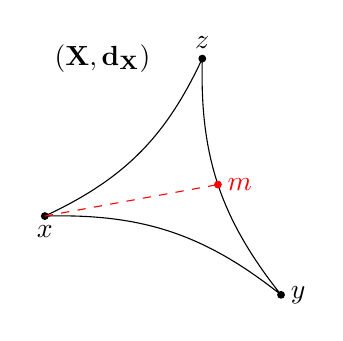
\begin{tikzpicture}[scale=1]
		\draw (0,1) node[fill,circle,inner sep=1pt]{}
		to [bend angle=20, bend left] (3,0) node[fill,circle,inner sep=1pt]{} 
		to [bend angle=20, bend left] coordinate[pos=.5] (M) (2,3) node[fill,circle,inner sep=1pt]{}
		to [bend angle=20, bend left] coordinate[pos=.33] (N) cycle;
		\draw (0,1) node[below]{$x$};
		\draw (3,0) node[right]{$y$};
		\draw (2,3) node[above]{$z$};
		\draw (M) node[fill,circle,inner sep=1pt,color=red]{};
		\draw (M) node[right,color=red]{$m$};
		\draw[color=red, dashed] (0,1) -- (M);
		\draw (0,3) node[right]{$\mathbf{(X,d_X)}$};
		\end{tikzpicture} \hspace{2cm}
		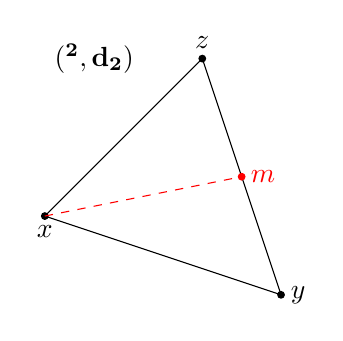
\begin{tikzpicture}[scale=1]
		\draw (0,1) node[fill,circle,inner sep=1pt]{}
		to (3,0) node[fill,circle,inner sep=1pt]{} 
		to coordinate[pos=.5] (M) (2,3) node[fill,circle,inner sep=1pt]{}
		to coordinate[pos=.33] (N) cycle;
		\draw (0,1) node[below]{$\ol{x}$};
		\draw (3,0) node[right]{$\ol{y}$};
		\draw (2,3) node[above]{$\ol{z}$};
		\draw (M) node[fill,circle,inner sep=1pt,color=red]{};
		\draw (M) node[right,color=red,xshift=-.2]{$\ol{m}$};
		\draw[color=red, dashed] (0,1) -- (M);
		\draw (0,3) node[right]{$\mathbf{(\RR^2,d_2)}$};
		\end{tikzpicture}	
	\end{figure}
\end{lemma}

\begin{satz}[Winkelbedingung für $\CAT$-Räume]
\label{satz:2.46}
	Sei $(X,d_X)$ ein geodätischer Raum.
	Dann sind äquivalent:
	\begin{enumerate}
		\item $X$ ist $\CAT$.
		\item Für jedes geodätische Dreieck $\Delta(x,y,z,\alpha,\beta,\gamma)$ in $X$ und Vergleichsdreieck $\ol{\Delta}(\ol{x},\ol{y},\ol{z})$ gilt $\angle(\alpha,\gamma) \leq \angle_{\ol{x}}(\ol{y},\ol{z})$.
	\end{enumerate}
\end{satz}

\begin{beweis}
	\mbox{} \\[-.9cm]
	\begin{description}
		\item[(i) $\Rightarrow$ (ii):] Sei $\Delta(x,y,z,\alpha,\beta,\gamma)$ ein beliebiges geodätisches Dreieck.
		Da $X$ $\CAT$ ist, gilt für $t \in [0,d(x,z)], t' \in [0,d(x,y)]$ beliebig:
		\[
			d(\alpha(t),\gamma(t')) \leq d_2(\ol{\alpha(t)},\ol{\gamma(t')}).
		\]
		\begin{figure}[h]
			\centering
			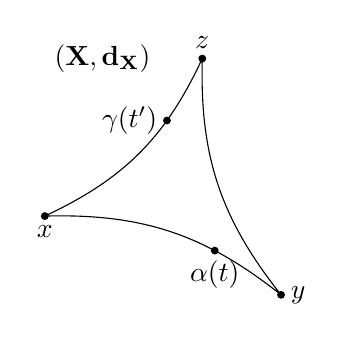
\begin{tikzpicture}[scale=1]
			\draw (0,1) node[fill,circle,inner sep=1pt]{}
			to [bend angle=20, bend left] coordinate[pos=.7] (A) (3,0) node[fill,circle,inner sep=1pt]{} 
			to [bend angle=20, bend left] (2,3) node[fill,circle,inner sep=1pt]{}
			to [bend angle=20, bend left] coordinate[pos=.3] (G) cycle;
			\draw (0,1) node[below]{$x$};
			\draw (3,0) node[right]{$y$};
			\draw (2,3) node[above]{$z$};
			\draw (A) node[fill,circle,inner sep=1pt]{};
			\draw (A) node[below]{$\alpha(t)$};
			\draw (G) node[fill,circle,inner sep=1pt]{};
			\draw (G) node[left]{$\gamma(t')$};
			\draw (0,3) node[right]{$\mathbf{(X,d_X)}$};
			\end{tikzpicture} \hspace{2cm}
			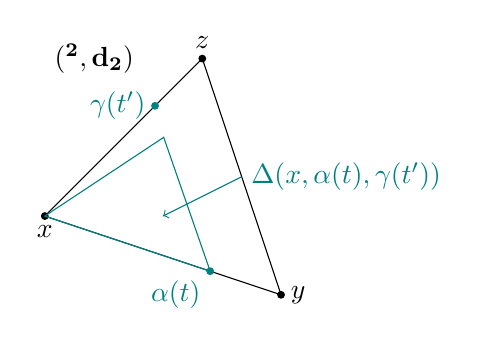
\begin{tikzpicture}[scale=1]
			\draw (0,1) node[fill,circle,inner sep=1pt]{}
			to coordinate[pos=.7] (A) (3,0) node[fill,circle,inner sep=1pt]{} 
			to (2,3) node[fill,circle,inner sep=1pt]{}
			to coordinate[pos=.3] (G) cycle;
			\draw (0,1) node[below]{$\ol{x}$};
			\draw (3,0) node[right]{$\ol{y}$};
			\draw (2,3) node[above]{$\ol{z}$};
			\draw [color=teal] (A) node[fill,circle,inner sep=1pt]{};
			\draw [color=teal] (G) node[fill,circle,inner sep=1pt]{};
			\draw [color=teal] (G) node[left]{$\ol{\gamma(t')}$};
			\draw [color=teal] (0,1) -- (A) node[anchor=north east]{$\ol{\alpha(t)}$} -- (1.51,2) -- cycle;			
			\draw [color=teal] (2.5,1.5) node[right]{$\ol{\Delta}(\ol{x},\ol{\ol{\alpha(t)}},\ol{\ol{\gamma(t')}})$};
			\draw [->,color=teal] (2.5,1.5) -- (1.5,1);
			\draw (0,3) node[right]{$\mathbf{(\RR^2,d_2)}$};
			\end{tikzpicture}	
		\end{figure}
		
		
		Folglich gilt $\angle_{\ol{x}}(\ol{\ol{\alpha(t)}},\ol{\ol{\gamma(t')}}) \leq \angle_{\ol{x}}(\ol{y},\ol{z})$ und damit
		\begin{align*}
			\angle(\alpha,\gamma) :&= \limsup\limits_{t,t' \rightarrow \infty} \angle_{\ol{x}}(\ol{\ol{\alpha(t)}},\ol{\ol{\gamma(t')}}) \\
			&\leq \limsup\limits_{t,t' \rightarrow \infty} \angle_{\ol{x}}(\ol{z},\ol{y}) \\
			&= \angle_{\ol{x}} (\ol{z},\ol{y})
		\end{align*}
		\item[(ii) $\Rightarrow$ (i):] Sei $\Delta(x,y,z,\alpha,\beta,\gamma)$ ein beliebiges geodätisches Dreieck in $X$.
		Wir zeigen, dass dann mit $m := \beta\enbrace*{\frac{d(z,y)}{2}}$ und Vergleichspunkt $\ol{m} := \ol{\beta}\enbrace*{\frac{d(\ol{z},\ol{y})}{2}}$ gilt:
		\[
			d(x,m) \leq d_2(\ol{x},\ol{m}).
		\]
		Dann folgt mit \autoref{lemma:2.45}, dass $X$ $\CAT$ ist.
		\newpage
		Wähle eine Geodäte zwischen $x$ und $m$ und betrachte die beiden schraffierten Dreiecke: 
		
		\begin{figure}[h]
			\centering
			\begin{tikzpicture}[scale=1.5,>=Latex]
				\draw (0,1) node[fill,circle,inner sep=1pt]{}
				to [bend angle=20, bend left] (3,0) node[fill,circle,inner sep=1pt]{} 
				to [bend angle=20, bend left] coordinate[pos=.5] (M) (2,3) node[fill,circle,inner sep=1pt]{}
				to [bend angle=20, bend left] cycle;
				\draw (0,1) node[below]{$x$};
				\draw (3,0) node[right]{$y$};
				\draw (2,3) node[above]{$z$};
				\draw (M) node[fill,circle,inner sep=1pt]{};
				\draw [->] (0,1) -- (M) node[right]{$m$};
				\draw (0,3) node[right]{$\mathbf{(X,d_X)}$};
				\draw [schraffiert=red] (0,1) to [bend angle=20, bend left] (3,0)
				to [bend angle=10, bend left] (M) to cycle;
				\draw [schraffiert=blue] (0,1) to (M) to [bend angle=10, bend left] (2,3)
				to [bend angle=20, bend left] cycle;
				\draw (1.5,1.2) node[above]{$\mathfrak{a}$};
				\draw (1.5,0.8) node[below]{$\alpha$};
				\draw (2.1,2) node[right]{$\beta$};
				\draw (1,1.7) node[above]{$\gamma$};
			\end{tikzpicture}
		\end{figure}
		
		Bezeichne mit $\mathfrak{a}$ die Geodäte von $x$ nach $m$.
		Wir haben zwei Möglichkeiten für die Lage von $\ol{\ol{m}}$ für die Vergleichsdreiecke $\ol{\Delta}(\ol{x},\ol{\ol{m}},\ol{\ol{z}})$ und $\ol{\Delta}(\ol{x},\ol{\ol{y}},\ol{\ol{m}})$:
		
		\begin{figure}[h]
			\centering
			\begin{tikzpicture}[scale=1.5,>=Latex]
				\draw (1.5,1.5) coordinate (M) node[right]{$\ol{\ol{m}}$} -- (0,1) coordinate (X) node[below]{$\ol{x}$} -- (3,0) coordinate (Y) node[below]{$\ol{\ol{y}}$} -- (M) -- (2,3) coordinate (Z) node[above]{$\ol{\ol{z}}$} -- (X);
				\draw pic[draw=black,angle radius=0.5cm]{angle=X--M--Y};
				\draw pic[draw=black,angle radius=0.5cm]{angle=Z--M--X};
			\end{tikzpicture} \hspace{2cm}
			\begin{tikzpicture}[scale=1.5,>=Latex]
			\draw (3,2) coordinate (M) node[right]{$\ol{\ol{m}}$} -- (0,1) coordinate (X) node[below]{$\ol{x}$} -- (3,0) coordinate (Y) node[below]{$\ol{\ol{y}}$} -- (M) -- (2,3) coordinate (Z) node[above]{$\ol{\ol{z}}$} -- (X);
			\draw pic[draw=black,angle radius=0.5cm]{angle=X--M--Y};
			\draw pic[draw=black,angle radius=0.5cm]{angle=Z--M--X};
			\end{tikzpicture}
		\end{figure}
		
		Für die Dreiecke $\Delta(x,m,z)$ und $\Delta(x,y,m)$ gilt (i).
		Wir haben also
		\[
			\angle(\beta\big|\_,\ol{\mathfrak{a}}) \leq \angle_{\ol{\ol{m}}}(\ol{x},\ol{\ol{z}}) \qquad \qquad \angle(\ol{\mathfrak{a}},\ol{\beta}\big|\_) \leq \angle_{\ol{\ol{m}}}(\ol{x},\ol{\ol{y}}),
		\]
		wobei $\ol{\mathfrak{a}},\ol{\beta}$ hier die inversen Geodäten bezeichnen.
		Wir erhalten:
		\begin{align*}
			&\angle_{\ol{\ol{m}}}(\ol{x},\ol{\ol{z}}) + \angle_{\ol{\ol{m}}}(\ol{x},\ol{\ol{y}}) \\
			\stack{}{\geq} &\angle(\beta\big|\_,\ol{\mathfrak{a}}) + \angle(\ol{\mathfrak{a}},\ol{\beta}\big|\_) \\
			\stack{\ref{prop:2.43}}{\geq} &\angle(\beta\big|\_,\ol{\beta}\big|\_) \stack{\ref{bsp:2.42}}{=} \pi.
		\end{align*}
		Also ist das Vergleichsdreieck von der Gestalt wie links.		
		Mit \autoref{lemma:2.44} folgt:
		\[
			d(x,m) = d_2(\ol{x},\ol{\ol{m}}) \leq d_2(\ol{x},\ol{m}). \qedhere
		\]
	\end{description}
\end{beweis}

\begin{satz}
\label{satz:2.47}
	Sei $Y$ ein lokaler $\CAT$-Raum.
	Weiter sei $Y$ eindeutig geodätisch und die Geodäten hängen stetig von ihren Endpunkten ab.
	Dann ist $Y$ ein $\CAT$-Raum.
\end{satz}

\begin{beweis}
	Wir zeigen die Winkelbedingung für $\CAT$-Räume.
	Seien $p,q_0,q_1 \in Y$ paarweise verschiedene Punkte und $\Delta(p,q_0,q_1)$ das geodätische Dreieck.
	Sei
	\[
		\begin{array}{l}
			q\colon [0,1] \rightarrow Y \text{ die linear umparametrisierte Geodäte von } q_0 \text{ nach } q_1, \\
			\beta\colon [0,1] \rightarrow Y \text{ die linear umparametrisierte Geodäte von } p \text{ nach } q_0 \text{ und} \\
			\gamma\colon [0,1] \rightarrow Y \text{ die linear umparametrisierte Geodäte von } p \text{ nach } q_1.
		\end{array}
	\]
	\begin{figure}[h]
		\centering
		\begin{tikzpicture}[scale=1.5,>=Latex]
			\draw [->] (0,0) coordinate (q0) node[below]{$q_0$}
			to [bend angle=10,bend left] coordinate[pos=.6] (qs) (4,0) coordinate (q1) node[below]{$q_1$};
			\draw [->] (2,3) coordinate (p) node[above]{$p$} to[bend angle=10,bend right] coordinate[pos=.1] (A) (q1) ;
			\draw [->] (p) to[bend angle=10,bend left] coordinate[pos=.1] (B) (q0);
			\draw [->,thick,color=teal] (p) to [bend angle=10,bend right] (qs) node[below]{$q(s)$};
			\draw pic["$\alpha$",draw=black,angle eccentricity=.7,angle radius=1cm]{angle=B--p--A};
			
			\draw (q0) node[fill,circle,inner sep=1pt]{};
			\draw (q1) node[fill,circle,inner sep=1pt]{};
			\draw (p) node[fill,circle,inner sep=1pt]{};
			\draw [color=teal] (qs) node[fill,circle,inner sep=1pt]{};
			
			\draw (1.5,.2) node[below]{$q$};
			\draw (3,1.25) node[right]{$\gamma$};
			\draw (1,1.25) node[left]{$\beta$};
			\draw [color=teal] (2.2,1) node[right]{$c_s$};			
		\end{tikzpicture}
	\end{figure}
	
	Zu zeigen ist:
	\[
		\alpha := \angle(\beta,\gamma) \leq \angle_{\ol{p}}(\ol{q_0},\ol{q_1}).
	\]
	Für $s \in [0,1]$ sei $c_s \colon [0,1] \rightarrow Y$ die linear umparametrisierte Geodäte von $p$ zu $q(s)$.
	Wir definieren
	\begin{align*}
		c\colon [0,1] \times [0,1] &\longrightarrow Y \\
		(s,t) &\longmapsto c_s(t)
	\end{align*}
	\begin{itemize}
		\item $c$ ist stetig, da die Geodäten in $Y$ stetig von ihren Endpunkten abhängen.
		\item $\im(c) \subseteq Y$ ist kompakt und $Y$ ist lokal $\CAT$, somit ist
		\[
			\im(c) \subseteq B_{\varepsilon_1}(p_1) \cup \dots \cup B_{\varepsilon_n}(p_n)
		\]
		mit $B_{\varepsilon_i}(p_i)$ $\CAT$.
		\item Wähle Unterteilungen
		\[
			\begin{array}{c}
				0  = s_0 < s_1 < \dots < s_k = 1 \\
				0 = t_0 < t_1 < \dots < t_l = 1
			\end{array}
		\]
		mit $c([s_i,s_{i+1}] \times [t_j,t_{j+1}]) \subseteq B_{\varepsilon_m}(p_m)$ für $m \in \{1,\dots,n\}$.
	\end{itemize}
	\begin{figure}[h]
		\centering
		\begin{tikzpicture}[scale=1,>=Latex]
			\draw [step=1] (0,0) grid (4,4);
			\draw (0,0) node[below]{$0$};
			\draw (1,0) node[below]{$s_1$};
			\draw (2,0) node[below]{$s_2$};
			\draw (3,0) node[below]{$s_3$};
			\draw (4,0) node[below]{$1$};
			\draw (0,1) node[left]{$t_1$};
			\draw (0,2) node[left]{$t_2$};
			\draw (0,3) node[left]{$t_3$};
			\draw (0,4) node[left]{$1$};
			\draw [schraffiert=teal] (2,2) -- (2,3) -- (3,3) -- (3,2) -- cycle;
			
			\draw [thick] (7,0) coordinate (q0) node[below]{$q_0$}
			to [bend angle=10,bend left] (11,0) coordinate (q1) node[below]{$q_1$};
			\draw [thick] (9,3) coordinate (p) node[above]{$p$} to[bend angle=10,bend right] (q1) ;
			\draw [thick] (p) to[bend angle=10,bend left] (q0);
					
			\draw (q0) node[fill,circle,inner sep=1pt]{};
			\draw (q1) node[fill,circle,inner sep=1pt]{};
			\draw (p) node[fill,circle,inner sep=1pt]{};
					
			\draw [schraffiert=teal] (8,1) circle (.6);
			\draw (9,2) circle (1.2);
			\draw (7.5,0) circle (.8);
			\draw (9.2,0.2) circle (1.2);
			\draw (10.5,1) circle (1.2);
			
			\draw [color=teal,->, thick] (3.1,2.5) to[bend angle=15,bend left] (7.3,1.1);
			\draw [color=teal] (5.5,2) node[above]{$c$};
			\end{tikzpicture}
	\end{figure}
	
	\begin{description}
		\item[0. Fall:] $k=1, l=1$. Nichts zu zeigen.
		\item[1. Fall:] $k=2, l =2$.
	\begin{figure}[h]
		\centering
		\begin{tikzpicture}[scale=1,>=Latex]
			\draw (1.5,0) node[below]{$s_1$} -- (1.5,4) -- (0,4) node[left]{$1$} -- (0,0) node[below]{$0$} -- (4,0) node[below]{$1$} -- (4,4) -- (1.5,4);
		\end{tikzpicture} \hspace{2cm}
		\begin{tikzpicture}[scale=1.5,>=Latex]
			\draw [->,thick] (0,0) coordinate (q0) node[below]{$q_0$}
			to [bend angle=10,bend left] coordinate[pos=.55] (qs) (4,0) coordinate (q1) node[below]{$q_1$};
			\draw [->,thick] (2,3) coordinate (p) node[above]{$p$} to[bend angle=10,bend right] coordinate[pos=.1] (A) (q1) ;
			\draw [->,thick] (p) to[bend angle=10,bend left] coordinate[pos=.1] (B) (q0);
			\draw [->,thick,color=teal] (p) to [bend angle=10,bend right] coordinate[pos=.1] (C) (qs) node[below]{$q(s_1)$};
			\draw pic["$\alpha_1$",draw=black,angle eccentricity=.8,angle radius=1.2cm]{angle=B--p--C};
			\draw pic["$\alpha_2$",draw=black,angle eccentricity=.8,angle radius=1.2cm]{angle=C--p--A};
			\draw pic["$\alpha$",draw=black,angle eccentricity=.9,angle radius=1.8cm]{angle=B--p--A};
			
			\draw (q0) node[fill,circle,inner sep=1pt]{};
			\draw (q1) node[fill,circle,inner sep=1pt]{};
			\draw (p) node[fill,circle,inner sep=1pt]{};
			\draw [color=teal] (qs) node[fill,circle,inner sep=1pt]{};
			
			\draw (1.5,.2) node[below]{$q$};
			\draw (3,1.25) node[right]{$\gamma$};
			\draw (1,1.25) node[left]{$\beta$};
			\draw (1.8,1) node[left]{$\Delta_1$};
			\draw (2.2,1) node[right]{$\Delta_2$};
			
			\draw (1.1,1.5) circle (1.8);			
			\draw (2.7,1.4) circle (1.8);
		\end{tikzpicture}
	\end{figure}
	Die $\CAT$-Winkelbedingung gilt für $\Delta_1$ und $\Delta_2$.
	\begin{align*}
		\angle(\beta,\gamma) &\stack{\ref{prop:2.43}}{\leq} \angle(\beta,c_{s_1}) + \angle(c_{s_1},\gamma) \\
		&\stack{\ref{satz:2.46}}{\leq} \angle_{\ol{p}} (\ol{\ol{q_0}},\ol{\ol{q(s_1)}}) + \angle_{\ol{p}}(\ol{\ol{q(s_1)}},\ol{\ol{q_1}}) \\
		&\stack{\ref{lemma:2.44}}{\leq} \angle_{\ol{p}}(\ol{q_0},\ol{q_1})
	\end{align*}
	\item[2. Fall:] $k=1, l > 1$.
		\begin{figure}[h]
			\centering
			\begin{tikzpicture}[scale=1,>=Latex]
				\draw (0,0) node[below]{$0 = s_0$} -- (4,0) node[below]{$1 = s_1$};
				\draw (0,1) node[left]{$t_1$} -- (4,1);
				\draw (0,2) node[left]{$t_2$} -- (4,2);
				\draw (0,3) node[left]{$t_3$} -- (4,3);
				\draw (0,4) node[left]{$1$} -- (4,4);
				\draw (0,0) -- (0,4);
				\draw (4,0) -- (4,4);
			\end{tikzpicture} \hspace{2cm}
			\begin{tikzpicture}[scale=1.5,>=Latex]
				\draw [thick] (0,0) coordinate (q0) node[below]{$q_0=c(0,1)$}
				to [bend angle=10,bend left] (4,0) coordinate (q1) node[below]{$q_1$};
				\draw [thick] (2,3) coordinate (p) node[above]{$p$} to[bend angle=10,bend right] coordinate[pos=.25] (P5) coordinate[pos=.5] (P3) coordinate[pos=.75] (P1) (q1);
				\draw [thick] (p) to[bend angle=10,bend left] coordinate[pos=.2] (P6) coordinate[pos=.45] (P4) coordinate[pos=.7] (P2) (q0);
				
				\draw (q0) node[fill,circle,inner sep=1pt]{};
				\draw (q1) node[fill,circle,inner sep=1pt]{};
				\draw (p) node[fill,circle,inner sep=1pt]{};
				\draw [color=teal] (P1) node[fill,circle,inner sep=1pt]{};
				\draw [color=teal] (P2) node[fill,circle,inner sep=1pt]{};
				\draw [color=teal] (P3) node[fill,circle,inner sep=1pt]{};
				\draw [color=teal] (P4) node[fill,circle,inner sep=1pt]{};
				\draw [color=teal] (P5) node[fill,circle,inner sep=1pt]{};
				\draw [color=teal] (P6) node[fill,circle,inner sep=1pt]{};
				
				\draw [color=teal] (P1) node[right]{$c(1,t_3)$};
				\draw [color=teal] (P3) node[right]{$c(1,t_2)$};
				\draw [color=teal] (P5) node[right]{$c(1,t_1)$};
				\draw [color=teal] (P2) node[left]{$c(0,t_3)$};
				\draw [color=teal] (P4) node[left]{$c(0,t_2)$};
				\draw [color=teal] (P6) node[left]{$c(0,t_1)$};
				
				\draw [thick,color=teal] (q0) -- (P1) -- (P2) -- (P3) -- (P4) -- (P5) -- (P6);
				\draw [color=teal] (2,2.5) node{$\Delta_1$};
				\draw [color=teal] (1.75,2) node{$\Delta_2$};
				\draw [color=teal] (2.25,1.75) node{$\Delta_3$};
				\draw [color=teal] (1.5,1.25) node{$\Delta_4$};
				\draw [color=teal] (2.5,1) node{$\Delta_5$};
				\draw [color=teal] (1,.5) node{$\Delta_6$};
				\draw [color=teal] (3.25,.4) node{$\Delta_7$};
			\end{tikzpicture}
		\end{figure}
		Verbinde die Punkte $c(s_i,t_j)$ mit Geodäten, wie im Bild zu sehen.
		Die $\CAT$-Winkelbedingung gilt für alle $\Delta_i$ so wie oben.
		Wende Fall 1 an auf das zusammengesetzte Dreieck bestehend aus $\Delta_1$ und $\Delta_2$.
		Demzufolge gilt die Winkelbedingung für das Dreieck $\Delta(p,c(0,t_2),c(1,t_1)$.
		Durch Wiederholung dieser Argumentation haben wir nach endlich vielen Schritten gezeigt, dass die Winkelbedingung für das Dreieck $\Delta(p,q_0,q_1)$ gilt.
		\newpage
		\item[3. Fall:] $k > 1, l > 1$.
		
		\begin{figure}[h]
			\centering
			\begin{tikzpicture}[scale=1.5,>=Latex]
			\draw [thick] (0,0) coordinate (q0) node[below]{$q_0$}
			to [bend angle=10,bend left] coordinate[pos=.25] (A1) coordinate[pos=.5] (A2) coordinate[pos=.75] (A3) (4,0) coordinate (q1) node[below]{$q_1$};
			
			\draw [thick] (2,3) coordinate (p) node[above]{$p$} to[bend angle=5,bend left] coordinate[pos=.2] (P7) coordinate[pos=.4] (P5) coordinate[pos=.6] (P3) coordinate[pos=.8] (P1) (A1);
			\draw [thick] (p) to[bend angle=10,bend left] coordinate[pos=.25] (P6) coordinate[pos=.5] (P4) coordinate[pos=.75] (P2) (q0);
			\draw [thick] (p) -- (A2);
			\draw [thick] (p) to[bend angle=5,bend right] (A3);
			\draw [thick] (p) to[bend angle=10,bend right] (q1);
			
			\draw (q0) node[fill,circle,inner sep=1pt]{};
			\draw (q1) node[fill,circle,inner sep=1pt]{};
			\draw (p) node[fill,circle,inner sep=1pt]{};
			
			\draw [thick,color=teal] (q0) -- (P1) -- (P2) -- (P3) -- (P4) -- (P5) -- (P6) -- (P7);
			\end{tikzpicture}
		\end{figure}
		
		Wende Fall 2 auf jede \enquote{Spalte} des Dreiecks an.
		Anschließend ist Fall 1 benutzbar. \qedhere
	\end{description}
\end{beweis}

\begin{definition}[konvex]
\label{def:2.48}
	\mbox{} \\[-1.4cm]
	\begin{enumerate}[(i)]
		\item Sei $I \subseteq \RR$ ein Intervall.
		Eine Funktion $\Phi\colon I \rightarrow \RR$ heißt \Index{konvex}, wenn für alle $t,s \in I$ und $\lambda \in [0,1]$ gilt: \marginnote{13.01. \\ \ [15]}
		\[
			\Phi(\lambda s + (1-\lambda)t) \leq \lambda \Phi(s) + (1-\lambda)\Phi(t).
		\]
		\item Sei $X$ ein geodätischer Raum.
		Eine Funktion $f \colon X \rightarrow \RR$ heißt \Index{konvex}, wenn für alle linear umparametrisierten Geodäten $c \colon [0,1] \rightarrow X$ die Funktion
		\begin{align*}
			\Phi \colon [0,1] &\longrightarrow \RR \\
			t &\longmapsto f(c(t))
		\end{align*}
		konvex ist.
	\end{enumerate}
\end{definition}
\newpage
\begin{lemma}
\label{lemma:2.49}
	Sei $X$ ein geodätischer Raum und $f \colon X \rightarrow \RR$ eine Funktion.
	Die Funktion $f$ ist genau dann konvex, wenn für alle linear umparametrisierten Geodäten $c \colon [0,1] \rightarrow X$ und $\lambda \in [0,1]$ gilt:
	\[
		f(c(\lambda)) \leq (1-\lambda) f(c(0)) + \lambda f(c(1)).
	\]
\end{lemma}

\begin{beispiel}
\label{bsp:2.50}
	Sei $(X,d)$ ein $\CAT$-Raum.
	Dann ist $d\colon X \times X \rightarrow \RR_{\geq 0}$ konvex, denn:
	
	Sei $c \colon [0,1] \rightarrow X \times X$ eine linear umparametrisierte Geodäte.
	Dann sind $\pi_1 \circ c \colon [0,1] \rightarrow X$  und $\pi_2 \circ c \colon [0,1] \rightarrow X$ linear umparametrisierte Geodäten, wobei $\pi_1$ bzw. $\pi_2$ Projektionen auf die erste bzw. zweite Komponente sind.
	Sei $\lambda \in [0,1]$ beliebig.
	Wir haben:
	\begin{align*}
		d(c(\lambda)) &\stack{}{=} d(\pi_1 \circ c(\lambda), \pi_2 \circ c(\lambda)) \\
		&\stack{\ref{aufg:1.2}}{\leq} (1-\lambda) \cdot d(\pi_1 \circ c(0),\pi_2 \circ c(0)) + \lambda \cdot d(\pi_1 \circ c(1), \pi_2 \circ c(1)) \\
		&\stack{}{=} (1-\lambda) \cdot d(c(0)) + \lambda \cdot d(c(1))
	\end{align*}
	Mit \autoref{lemma:2.49} folgt, dass $d \colon X \times X \rightarrow \RR_{\geq 0}$ konvex ist.
\end{beispiel}

\begin{definition}[lokal konvex]
\label{def:2.51}
	Sei $I \subseteq \RR$ ein Intervall.
	Eine Funktion $\Phi \colon I \rightarrow \RR$ heißt \textbf{lokal konvex}, wenn für alle $\lambda \in I$ ein $\varepsilon_\lambda > 0$ existiert, sodass $\Phi \big|_{B_{\varepsilon_\lambda}(\lambda)} \colon B_{\varepsilon_\lambda}(\lambda) \cap I \rightarrow \RR$ konvex ist. \index{konvex!lokal}
\end{definition}

\begin{lemma}
\label{lemma:2.52}
	Sei $\Phi\colon [0,1] \rightarrow \RR$ eine lokal konvexe Funktion.
	Dann ist $\Phi$ konvex. (\autoref{aufg:7.1})
\end{lemma}

Es folgt nun der Beweis von \autoref{lemma:2.32}.

\begin{beweis}
\label{bew:tech_lemma}
	Da $X$ lokal $\CAT$ und lokal vollständig ist, existiert für jedes $x \in X$ ein $r_x > 0$, sodass $B_{r_x}(x) \CAT$ ist und $\ol{B_{r_x}(x)}$ vollständig ist.
	Wir betrachten nun die offene Überdeckung
	\[
		c([0,1]) \subseteq \bigcup_{t \in [0,1]} B_{\frac{r_{c(t)}}{2}}(c(t)).
	\]
	Weiter ist $[0,1]$ kompakt und $c \colon [0,1] \rightarrow X$ ist stetig.
	Folglich ist $c([0,1])$ kompakt.
	Es existieren also $t_1, \dots, t_n \in [0,1]$ mit
	\begin{equation}
		c([0,1]) \subseteq B_{\frac{r_{c(t_1)}}{2}}(c(t_1)) \cup \dots \cup B_{\frac{r_{c(t_n)}}{2}}(c(t_n)). \label{eq:bew_tl_1}
	\end{equation}
	Wir definieren nun
	\[
		\varepsilon := \frac{\min\{r_c(t_1), \dots r_c(t_n)\}}{4}.
	\]
	Für alle $t \in [0,1]$ gilt nun, dass $B_{2\varepsilon}(c(t)) \CAT$ und $\ol{B_{2\varepsilon}(c(t))}$ vollständig ist, denn:
	
	Sei $t \in [0,1]$ belieibg.
	Dann existiert nach \eqref{eq:bew_tl_1} ein $i \in \{1, \dots, n\}$ mit $c(t) \in B_{\frac{r_c(t_i)}{2}}(c(t_i))$.
	Wir zeigen $B_{2\varepsilon}(c(t)) \subseteq B_{r_c(t_i)}(c(t_i))$.
	
	Sei also $x \in B_{2\varepsilon}(c(t))$ beliebig.
	Es gilt:
	\begin{align*}
		d(x,c(t_i)) &\stack{\Delta\text{-Ungl.}}{\leq} d(x,c(t)) + d(c(t),c(t_i)) \\
		&\stack{}{<} 2\varepsilon + \frac{r_{c(t_i)}}{2} \\
		&\stack{}{\leq} 2 \cdot \frac{r_c(t_i)}{4} + \frac{r_{c(t_i)}}{2} = r_{c(t_i)}
	\end{align*}
	Folglich ist $x \in B_{r_{c(t_i)}} (c(t_i))$.
	
	Zur Konvexitätsaussage und Eindeutigkeit von $c_{\ol{x},\ol{y}}$:
	Seien $c_1,c_2 \colon [0,1] \rightarrow X$ linear umparametrisierte lokale Geodäten mit $\sup_{t \in [0,1]} d(c_i(t),c(t)) < \varepsilon$ für $i = 1,2$.
	Wir betrachten nun die Funktion
	\begin{align*}
		\Phi\colon [0,1] &\longrightarrow \RR_{\geq 0} \\
		t &\longmapsto d(c_1(t),c_2(t)).
	\end{align*}
	$\Phi$ ist konvex:
	Sei $t \in [0,1]$ beliebig.
	Es existiert $\varepsilon_1', \varepsilon_2' > 0$, sodass
	\begin{align*}
		c_1 \colon [t- \varepsilon_1', t+ \varepsilon_1'] &\longrightarrow B_{2\varepsilon}(c(t)) \\
		c_2 \colon [t-\varepsilon_2', t+\varepsilon_2'] &\longrightarrow B_{2\varepsilon}(c(t)),
	\end{align*}
	und $B_{2\varepsilon}(c(t))$ ist $\CAT$.
	Wir definieren $\varepsilon' := \min\{ \varepsilon_1',\varepsilon_2'\}$.
	Nach \autoref{aufg:2.1} sind lokale Geodäten in $\CAT$-Räumen schon globale Geodäten.
	Folglich sind  $c_1 \big|_{[t-\varepsilon',t+\varepsilon']}$ und $c_2 \big|_{[t-\varepsilon',t+\varepsilon']}$ linear umparametrisierte Geodäten.
	Nach \autoref{bsp:2.50} ist
	\[
	d \big|_{B_{2\varepsilon}(c(t))} \colon B_{2\varepsilon}(c(t)) \times B_{2\varepsilon}(c(t)) \rightarrow \RR_{\geq 0}
	\]
	eine konvexe Funktion. Folglich ist $\Phi \colon [t- \varepsilon',t+\varepsilon'] \rightarrow \RR_{\geq 0}$ konvex.
	Mit \autoref{lemma:2.52} folgt, dass $\Phi$ global konvex ist.
	
	Damit können wir nur die Eindeutigkeit zeigen:
	Seien $\ol{x} \in B_\varepsilon(x), \ol{y} \in B_\varepsilon(y)$ beliebig und $c_{\ol{x},\ol{y}}, c_{\ol{x},\ol{y}}' \colon [0,1] \rightarrow X$ linear umparametrisierte Geodäten von $\ol{x}$ nach $\ol{y}$ mit der Eigenschaft
	\begin{align*}
		\sup_{t\in [0,1]} d(c_{\ol{x},\ol{y}}, c(t)) &\stack{}{<} \varepsilon \\
		\sup_{t \in [0,1]} d(c_{\ol{x},\ol{y}}',c(t)) &\stack{}{<} \varepsilon.
	\end{align*}
	Wir wissen, dass die Funktion
	\begin{align*}
		\Phi\colon [0,1] &\longrightarrow \RR_{\geq 0} \\
		t &\longmapsto d(c_{\ol{x},\ol{y}}(t),c_{\ol{x},\ol{y}}'(t))
	\end{align*}
	konvex ist. \newpage
	Insbesondere gilt für $\lambda \in [0,1]$ beliebig:
	\begin{align*}
		\Phi(\lambda) &\leq (1-\lambda) \Phi(0) + \lambda \cdot \Phi(1) \\
		d(c_{\ol{x},\ol{y}}(\lambda),c_{\ol{x},\ol{y}}'(\lambda)) &\leq (1-\lambda) \cdot d(c_{\ol{x},\ol{y}}(0),c_{\ol{x},\ol{y}}'(0)) + \lambda \cdot d(c_{\ol{x},\ol{y}}(1),c_{\ol{x},\ol{y}}'(1)) \\
		&\leq (1-\lambda) \cdot d(\ol{x},\ol{x}) + \lambda \cdot d(\ol{y},\ol{y}) = 0
	\end{align*}
	Folglich erhalten wir $c_{\ol{x},\ol{y}}(\lambda) = c_{\ol{x},\ol{y}}'(\lambda)$, also $c_{\ol{x},\ol{y}} = c_{\ol{x},\ol{y}}'$.
					
	Zur Existenz von $c_{\ol{x},\ol{y}}$:
	Wir definieren für $A \in (0,1]$ die \textbf{Eigenschaft P(A)}:
	Für alle $a,b \in [0,1]$ mit $0 < b-a \leq A$ und alle $\ol{p} \in B_\varepsilon(c(a)), \ol{q} \in B_\varepsilon(c(b))$ existiert eine linear umparametrisierte lokale Geodäte $c_{\ol{p},\ol{q}} \colon [a,b] \rightarrow X$ von $\ol{p}$ nach $\ol{q}$ mit
	\[
		\sup_{t \in [a,b]} d(c_{\ol{p},\ol{q}}(t),c(t)) < \varepsilon.
	\]
	Wir zeigen:
	\begin{enumerate}[(1)]
		\item Es existiert ein $A \in (0,1]$, sodass die Eigenschaft $P(A)$ wahr ist.
		\item Ist $P(A)$ wahr, dann auch $P(\frac{3A}{2})$.
	\end{enumerate}
	Dadurch folgt die Existenz von $c_{\ol{x},\ol{y}}$.
	
	\begin{enumerate}[(1)]
		\item Für $A = \frac{\varepsilon}{\ell(c)}$ gilt $P(A)$, denn:
		Seien $a,b \in [0,1]$ mit $0 < b-a \leq \frac{\varepsilon}{\ell(c)}$ beliebig.
		Dann ist
		\[
			d(c(a),c(b)) \leq \ell(c \big|_{[a,b]}) \stack{\CAT}{=} \ell(c) \cdot \abs{b-a} \leq \varepsilon,
		\]
		also ist $c\big|_{[a,b]}$ linear umparametrisierte Geodäte.
		Sei weiter $\ol{p} \in B_\varepsilon(c(a)), \ol{q} \in B_\varepsilon(c(b))$ beliebig.
		Dann gilt $\ol{p}, \ol{q} \in B_{2\varepsilon}(c(a))$.
		Da $B_{2\varepsilon}(c(a)) \CAT$ ist, existiert eine linear umparametrisierte Geodäte $c_{\ol{p},\ol{q}}$ von $\ol{p}, \ol{q}$.
		\item Seien $a,b \in [0,1]$ mit $0 < b-a \leq \frac{3}{2}A$ beliebig.
		Teile das Intervall $[a,b]$ in drei gleich große Intervalle $[a,a_1],[a_1,b_1],[b_1,b]$ auf. 		
		
		Sei weiter $\ol{p} \in B_\varepsilon(c(a))$ und $\ol{q} \in B_\varepsilon(c(b))$ beliebig.
		Wir definieren induktiv Folgen $p_n$ und $q_n$ in $X$:
		Setze $p_0 := c(a_1), q_0 := c(b_1)$.
		Seien $p_{n-1}, q_{n-1}$ bereits konstruiert.
		Da $P(A)$ gilt, existieren linear umparametrisierte lokale Geodäten $c_n \colon [a, b_1] \rightarrow X$ von $\ol{p}$ zu $q_{n-1}$ und $c_n' \colon [a_1,b] \rightarrow X$ von $p_{n-1}$ zu $\ol{q}$.
		Setze dann $p_n := c_n(a_1)$ und $q_n := c_n'(b_1)$. Es gilt (ohne Beweis -- nachrechnen):
		\begin{enumerate}[(i)]
			\item $(p_n)_{n \in \NN}, (q_n)_{n \in \NN}$ sind Cauchy-Folgen.
			\item $p_n \in \ol{B_\varepsilon(p_0)}, q_n \in \ol{B_\varepsilon(q_0)}$ sind vollständig für alle $n \in \NN$.
			Folglich sind $(p_n)_n, (q_n)_n$ konvergente Folgen.
			\item Für $t \in [a,b_1]$ $(c_n(t))_n$ eine Cauchy-Folge in $\ol{B_\varepsilon(c_(t))}$.
			Folglich ist $(c_n(t))_n$ eine konvergente Folge.
			\item Für $t \in [a_1,b]$ ist $(c_n'(t))_n$ eine Cauchy-Folge in $\ol{B_\varepsilon(c(t))}$.
			Folglich ist $(c_n'(t))_n$ eine konvergent Folge.
		\end{enumerate}
		
		\begin{figure}[h]
			\centering
			\begin{tikzpicture}[scale=2,>=Latex]
			\draw (0,-1.5) node[circle,fill,inner sep=1.5pt]{} to coordinate[pos=.333] (a) coordinate[pos=.8] (a1) (2.1,-1.5);
			\draw (2.1,-1.5) to coordinate[pos=.3] (b1) coordinate[pos=.85] (b) (4.2,-1.5) node[circle,fill,inner sep=1.5pt]{};
			
			\coordinate (x) at (0,-5);
			\coordinate (y) at (4.2,-5);
			
			\draw (x) to[bend angle=10,bend left] coordinate[pos=.333] (ca) coordinate[pos=.8] (p0) (2.1,-5) to [bend angle=10,bend right] coordinate[pos=.3] (q0) coordinate[pos=.85] (cb) (y);
			
			\coordinate (pbar) at (0,-2);
			\coordinate (qbar) at (4.2,-2);
			
			\draw [color=red] (pbar) to coordinate[pos=.6] (p1) (q0);
			\draw [color=red] (p1) node[anchor=north east]{$p_1$};
			\draw [color=red] (p1) node[fill,circle,inner sep=1.5pt]{};
			
			\draw [color=Green4] (p0) to coordinate[pos=.4] (q1) (qbar);
			\draw [color=Green4] (q1) node[anchor=north west]{$q_1$};
			\draw [color=Green4] (q1) node[fill,circle,inner sep=1.5pt]{};
			
			\draw [color=red] (pbar) to coordinate[pos=.6] (p2) (q1);
			\draw [color=red] (p2) node[anchor=north east]{$p_2$};
			\draw [color=red] (p2) node[fill,circle,inner sep=1.5pt]{};
			
			\draw [color=Green4] (p1) to coordinate[pos=.4] (q2) (qbar);
			\draw [color=Green4] (q2) node[anchor=north west]{$q_2$};
			\draw [color=Green4] (q2) node[fill,circle,inner sep=1.5pt]{};
			
			\draw [color=red] (pbar) to coordinate[pos=.6] (p3) (q2);
			\draw [color=red] (p3) node[anchor=north east]{$p_3$};
			\draw [color=red] (p3) node[fill,circle,inner sep=1.5pt]{};
			
			\draw [color=Green4] (p2) to coordinate[pos=.4] (q3) (qbar);
			\draw [color=Green4] (q3) node[anchor=north west]{$q_3$};
			\draw [color=Green4] (q3) node[fill,circle,inner sep=1.5pt]{};
			
			\draw [color=red] (pbar) to coordinate[pos=.6] (p4) (q3);
			\draw [color=red] (p4) node[fill,circle,inner sep=1.5pt]{};
			
			\draw [color=Green4] (p3) to coordinate[pos=.4] (q4) (qbar);
			\draw [color=Green4] (q4) node[fill,circle,inner sep=1.5pt]{};
			
			\draw [color=red] (pbar) to coordinate[pos=.6] (p5) (q4);
			\draw [color=red] (p5) node[fill,circle,inner sep=1.5pt]{};
			
			\draw [color=Green4] (p4) to coordinate[pos=.4] (q5) (qbar);
			\draw [color=Green4] (q5) node[fill,circle,inner sep=1.5pt]{};
			
			\draw [color=red] (pbar) to coordinate[pos=.6] (p6) (q5);
			\draw [color=red] (p6) node[fill,circle,inner sep=1.5pt]{};
			
			\draw [color=Green4] (p5) to coordinate[pos=.4] (q6) (qbar);
			\draw [color=Green4] (q6) node[fill,circle,inner sep=1.5pt]{};
			
			\draw [very thick,color=red] (pbar) -- (2.62,-2.01) node[fill,circle,inner sep=1.5,color=Green4]{};
			\draw [color=red] (1.365,-2) node[above]{$\mathbf{\alpha}$};
			
			\draw [very thick,color=Green4] (4.2,-1.99) -- (1.58,-1.99) node[fill,circle,inner sep=1.5,color=red]{};
			\draw [color=Green4] (2.94,-2) node[above]{$\mathbf{\beta}$};
			
			\foreach \x in {a,a1,b1,b,x,ca,p0,q0,cb,y,pbar,qbar} {
				\draw (\x) node[fill,circle,inner sep=1.5pt]{};
			}
			
			\draw (0,-1.5) node[above]{$0$};
			\draw (a) node[above]{$a$};
			\draw (a1) node[above]{$a_1$};
			\draw (b1) node[above]{$b_1$};
			\draw (b) node[above]{$b$};
			\draw (4.2,-1.5) node[above]{$1$};
			
			\draw (x) node[below]{$x$};
			\draw (ca) node[below]{$c(a)$};
			\draw (p0) node[below]{$c(a_1) = p_0$};
			\draw (q0) node[below]{$c(b_1) = q_0$};
			\draw (cb) node[below]{$c(b)$};
			\draw (y) node[below]{$y$};
			
			\draw (pbar) node[below]{$\ol{p}$};
			\draw (qbar) node[below]{$\ol{q}$};
			
			\draw [color=red] (.5,-2.5) node[anchor=north east]{$c_1$};
			\draw [color=Green4] (3.75,-2.5) node[anchor=north west]{$c_1'$};
			\end{tikzpicture}
		\end{figure}
		
		Wir definieren
		\begin{align*}
			\alpha \colon [a,b_1] &\longrightarrow X \\
			t &\longmapsto \lim\limits_{n \rightarrow \infty} c_n(t)
		\end{align*}
		und
		\begin{align*}
			\beta \colon [a_1,b] &\longrightarrow X \\
			t &\longmapsto \lim\limits_{n \rightarrow \infty} c_n'(t).
		\end{align*}
		Die Konvergenz $c_n \rightarrow \alpha$ und $c_n' \rightarrow \beta$ ist gleichmäßig und $\alpha$ und $\beta$ sind linear umparametrisierte lokale Geodäten.
		Weiter gilt $\alpha \big|_{[a_1,b_1]} = \beta \big|_{[a_1,b_1]}$.
		Die Komposition $\alpha\big|_{[a,a_2]} * \beta \big|_{[a_1,b]}$ ist die gesuchte linear umparametrisierte lokale Geodäte $c_{\ol{p},\ol{q}}$. \qedhere
	\end{enumerate}
\end{beweis}


\cleardoubleoddemptypage